% concatenated from main-for-arxiv.tex, mymacro.tex, intro.tex, comprehensive-en.tex, contiguity1.tex, contiguity2.tex, isom.tex, restriction.tex, gauss-hg.tex, appell1.tex, mybib.tex
%\documentclass[dvipdfmx]{jsarticle}
\documentclass{article}
\usepackage{color}
\usepackage{graphicx} % Required for inserting images
\usepackage{amsthm, amsmath,color,amssymb}
\usepackage{url}

\usepackage{tikz}
\usetikzlibrary{intersections,calc,arrows.meta,patterns}

\title{Comprehensive Restriction Algorithm for Hypergeometric Systems}
\author{Hiromasa Nakayama and Nobuki Takayama}
\date{August 29, 2025}

%\def\aa{\alpha}
%\def\bb{\beta}
%\def\cc{\gamma}
\def\aa{a}
\def\bb{b}
\def\cc{c}

\def\CC{\mathbb{C}}
\def\KK{{\bf K}}
\def\NN{\mathbb{N}}
\def\QQ{\mathbb{Q}}
\def\RR{\mathbb{R}}
\def\ZZ{\mathbb{Z}}
\def\memo#1{{\color{blue} #1}}
\def\p{\partial}
\def\pd#1{\partial_{#1}}
\def\qed{\hfill $\Box$ \medbreak}

\def\prog#1{{\tt #1}}

%%%%%%%%%%%%%%%%%%%%%%%%%%%%%%%%%%%%%%%%%%%%%%%%%
% for CGS
%%%%%%%%%%%%%%%%%%%%%%%%%%%%%%%%%%%%%%%%%%%%%%%%%
\def\CGS{{\rm CGS}}
\def\pp{{\rm pp}}
\def\lpp{{\rm lpp}}
\def\lc{{\rm lc}}
\def\lm{{\rm lm}}

\def\ppx{{\rm pp_{\{x,\p\}}}}
\def\lppx{{\rm lpp_{\{x,\p\}}}}
\def\lcx{{\rm lc_{\{x,\p\}}}}
\def\lmx{{\rm lm_{\{x,\p\}}}}
\def\MBlppx{{\rm MBlpp_{\{x,\p\}}}}

\def\id{{\rm Id}}

%% 省力化用
\def\aalpha{a}
\def\bbeta{b}
\def\ggamma{c}
%\def\Hg{H_{{}_2F_1}}
\def\Hg{H_g}


\newtheorem{definition}{Definition}
\newtheorem{theorem}{Theorem}
\newtheorem{proposition}{Proposition}
\newtheorem{example}{Example}
\newtheorem{algorithm}{Algorithm}
\newtheorem{remark}{Remark}



\begin{document}

\maketitle

\section{Introduction}

We denote by $D$ the Weyl algebra
$$\CC \langle x_1, \ldots, x_n, \pd{1}, \ldots, \pd{n} \rangle, $$
that is the ring of linear partial differential operators
with polynomial coefficients.
Let $M$ be a holonomic $D$-module 
on the $n$-dimensional space $\CC^n=\{ x=(x_1, \ldots, x_n) \}$.
The $0$-th restriction of $M$ to $V(x_{m+1}, \ldots, x_n)$ 
is defined as
$$
\frac{M}{x_{m+1}M + \cdots + x_n M}
$$
(see, e.g., \cite{bjork-2012}, \cite[Chap 5]{SST}).
An algorithm computing the restriction 
was given by T.Oaku \cite{oaku-1997}.
In this paper, we consider a problem of computing the restriction
for a given holonomic $D$-module with parameters.
We will give a partial answer to the problem for general holonomic $D$-modules
and an answer to hypergeometric holonomic $D$-modules.


The basic method for performing various calculations on ideals 
or submodules of free modules
involving parameters is 
the comprehensive Gr\"bner basis introduced 
by V.Weispfenning \cite{weispfenning-1992}.
K.Nabeshima, K.Ohara, S.Tajima \cite{not-2016} introduced comprehesive Gr\"obner systems
(CGS) for rings of linear partial differential operators.
They applied their method of computing CGS to the problem of computing
$b$-functions for polynomials with parameters.
The parameter space is stratified so that a $b$-function is associated
to each stratum.

For a given holonomic $D$-module with parameters,
we want to stratify the parameter space so that
a restriction module that does not depend on parameters
is associated to each stratum.
We start with generalizing the method by K.Nabeshita et al. 
to compute a generic $b$-function
that is also called an indicial polynomial or 
a $b$-function for restriction (Section \ref{sec:comprehensive}).
The maximal integral root of it plays the central role
to apply the Oaku's $b$-function criterion 
of the restriction algorithm \cite{oaku-1997}.
The parameter space can be stratified so that a generic $b$-function
is associated to each stratum.
However, the difficulty is that roots of it still depends on parameters.
We use isomorphic correspondences of D-modules with parameters
to address this difficulty.
Since we only need to consider integral roots to obtain the restriction, 
isomorphic correspondences are fully available.

We focus on algorithms to construct isomorphisms
among hypergeometric $D$-modules in sections \ref{sec:contiguity1},
\ref{sec:rat-sol}, \ref{sec:restriction_of_A_hg}, \ref{sec:isom}.
M.Saito gave an algorithm to classify GKZ hypergeometric systems
into isomorphic classes \cite{saito-isom}.
We give an algorithm to classify a class of hypergeometric systems of Horn type
\cite{berkesch} into isomorphic classes.
The key ingradient of our method is constructing strata so that
a contiguity relation of a hypergeometric system with parameters
is associated to each stratum.
Note that a general algorithm to check if two holonomic $D$-modules
are isomorphic or not is given by H.Tsai and U.Walther \cite{tw-hom}.
Considering a comprehensive version of this algorithm is a future problem.

Utilizing algorithms to classifying isomorphic classes
of hypergeometric systems, we finally give a comprehensive restriction
algorithm in section \ref{sec:restriction}.
The remaining sections \ref{sec:gauss-hg}, \ref{sec:f1} are discussions 
on restrictions to the origin
of the Gauss hypergeometric system and the Appell $F_1$ system.


%\input comprehensive
%%Note: 一般のパラメータは beta, 数としても不定元としても使う. Gauss その他の parameter は a,b,c.
\section{Comprehensive Gr\"obner System and Generic $b$-function} \label{sec:comprehensive}

K.Nabeshima, K.Ohara, S.Tajima introduced
an algorithm for computing comprehensive Gr\"obner systems (CGS) in rings of linear partial differential operators \cite{not-2016}.
They also gave applications of CGS for computing $b$-functions for singularities.
We apply their algorithm to obtain $b$-functions 
for weight vectors
to compute restrictions of $D$-modules. See, e.g., \cite[Chap 5]{SST} on $b$-functions for weight vectors. Being inspired by the computer algebra system 
Risa/Asir\footnote{\url{https://www.openxm.org}} command name
{\tt generic\_bfct}, we call them {\it generic $b$-functions}.
We also call a generic $b$-function {\it a $b$-function for restriction}
in this paper to distinguish with a $b$-function of a contiguity relation
and a $b$-function for a polynomial.

Let 
$$D_n[\beta]=\CC[\beta_1, \ldots, \beta_m]
  \langle x_1, \ldots, x_n, \pd{1}, \ldots, \pd{n} 
  \rangle
$$
be the Weyl algebra with parameters
$\beta=(\beta_1, \ldots, \beta_m)$
regarded as indeterminates.
We denote $D_n$ by $D$ when the number of variables is clear.
For a left ideal $I$ generated by a set
of generators $P$ in $D[\beta]$,
we compute a Gr\"obner basis $G$ with a block order
$\succ_b$
satisfying $x_i, \pd{i} \succ_b \beta_j$
for any $i$ and $j$
where $\succ$ is a tie-breaker of the block order.
Put $E=G \cap \CC[\beta]$ and $G'=G \setminus E$.
The set $V(E)$ is a given set of equality constraints on parameters.
We denote by $\CGS(E, N, P, \succ_b)$
or by $\CGS(E, N, I, \succ_b)$
the output CGS of $I$ on $V(E) \setminus V(N)$
where $N$ is a given set of equality constraints on parameters.
%where $N$ is a subset  of $\CC[\beta]$ by the algorithm given in \cite{not-2016}.
The CGS is a finite set of data of the form $(V(E_i) \setminus V(N_i), {\cal G}_i)$
where $E_i, N_i \subset \CC[\beta]$, ${\cal G}_i \subset D[\beta]$ and
they are finite set.
The CGS has a property that
for any $a \in V(E_i) \setminus V(N_i)$,
${\cal G}_i |_{\beta=a}$ is a Gr\"obner basis of $P|_{\beta=a}$ in $D$ 
with respect to the order $\prec$.
$V(E_i) \setminus V(N_i)$ is called a stratum % 単数, strata が pl.
and the strata of this form in the CGS cover $V(E) \setminus V(N)$.
Note that when $E=\emptyset$, we regard $V(E)=\CC^m$.
The procedure $\CGS$ is recursively called.
At the top level, we usually start with $\CGS(E=\emptyset,N=\{1\},P,\succ_b)$.
Note that $V(\{1\})=\emptyset$.
%In our applications, the procedure CGS is often applied under the condition $E \subset P$ and $G \cap \CC[\beta] = E$.

%\begin{example}[Appell $F_1, F_2$ の CGS]
%\end{example}

Let $w$ be a vector in $\ZZ_{\geq 0}^n$.
The $(-w,w)$-degree of $a x^p \pd{}^q$ 
is $-w\cdot p + w \cdot q$
where $a \in \CC[\beta_1, \ldots, \beta_m]$,
$a \not= 0$, and 
$x^p=\prod_{i=1}^n x_i^{p_i}$, 
$\pd{}^q=\prod_{i=1}^n \pd{i}^{q_i}$. 
The $(-w,w)$-initial term for 
$\ell=\sum_{(p,q)\in E} a_{pq} x^p \pd{}^q$
is the sum of the maximal $(-w,w)$-degree terms of $\ell$
and is denoted by 
${\rm in}_{(-w,w)}(\ell)$.
For a given left ideal $I$ in $D[\beta]$,
the ideal generated by ${\rm in}_{(-w,w)}(\ell)$, $\ell \in I$
is called {\it the initial form ideal} (with respect to the weight
vector $(-w,w)$.

Let $\succ$ is a term order in $D[\beta]$.
The order $\succ_{(-w,w)}$ is defined as
\begin{eqnarray*}
&&  c_{pq}(\beta) x^p \pd{}^q \succ_{(-w,w)}  c'_{p'q'}(\beta) x^{p'} \pd{}^{q'} \\
&\Leftrightarrow&
 -w\cdot p + w \cdot q >  -w\cdot p' + w \cdot q' \\
 & & \quad \mbox{ or } \ 
 (-w\cdot p + w \cdot q =  -w\cdot p' + w \cdot q' \ \mbox{ and } \ 
  x^p \pd{}^q \succ x^{p'} \pd{}^{q'}). 
\end{eqnarray*}
Since the order $\succ_{(-w,w)}$ is not a well-order,
we need to utilize the homogenized Weyl algebra to compute
Gr\"obner bases with this order.
Their CGS algorithm can also be applied 
to the homogenized Weyl algebra with parameters
(see, e.g., \cite[Th. 1.2.6]{SST} on the homogenized Weyl algebra),
%%todo [Oaku, Th.3.51]
and obtain a CGS for the initial form ideal
of a given left ideal in $D[\beta]$.
This method utilizing the homogenized Weyl algebra 
is not explicitly described in the paper \cite{not-2016}, 
so we explain it below.
Note that the case of the holonomic $D$-module $M$ is of the form
$D^m/I$ where $I$ is a submodule can be discussed analogously.
%%todo: precise description and implementation.

\begin{algorithm}[Computing parametric initial form ideal]\rm \label{alg:CGS}
~~
\begin{itemize}
\item
Input : a set of generators of a left ideal  $I$ 
in $D[\beta]$,~ a weight vector $w \in (\ZZ_{\geq 0})^n$
\item
Output : A stratification of the parameter space
$\{(E_i,N_i)\}$ and
generators of the initial form ideal ${\rm in}_{(-w,w)}(I)$ on the stratum $V(E_i) \setminus V(N_i)$.
\end{itemize}
\begin{enumerate}
\item
\if 0
Homogenize each element of the set of generators of $I$. 
We denote by $I^h$
the ideal generated by these homogenized element.
%% This method seems to be  a marking method
Let $h$ be the homogenization variable 
of weight $-1$.
Homogenize 
each element of the set of generators of $I$ 
with respect to the weight vector $(-w,w)$.
Precisely,
for $\ell = \sum_{p, q} c_{p, q} x^p \partial^q$,
put
$k_0 = {\rm min}\{ -w \cdot p + w \cdot q) \mid c_{p, q} \neq 0\}$
and homogenize $\ell$ as
$$
\ell^h = \sum_{p, q} c_{p, q} x^p \partial^q h^{-w\cdot p+w\cdot q - k_0}
$$
\fi

\item 
Let $\succ^h_{(-w,w)}$ be an order in the homogenized Weyl algebra
defined as 
\begin{eqnarray*}
&&  c_{pq}(\beta) x^p \pd{}^q h^r \succ^h_{(-w,w)}  c'_{p'q'}(\beta) x^{p'} \pd{}^{q'} h^{r'} \\
&\Leftrightarrow&
 -w\cdot p + w \cdot q >  -w\cdot p' + w \cdot q' \\
 & & \quad \mbox{ or } \ 
 (-w\cdot p + w \cdot q =  -w\cdot p' + w \cdot q' \ \mbox{ and } \ 
  x^p \pd{}^q h^r \succ x^{p'} \pd{}^{q'} h^{r'}). 
\end{eqnarray*}
where the tie-breaker is an elimination order of $h$.
Extending $\succ^h_{(-w,w)}$ to a block order $\succ^h_{b,(-w,w)}$
such that $x_i, \pd{i}, h \succ^h_{b,(-w,w)} \beta_j$,
we compute a CGS 
$$
\mathcal{G} = \{(E_i, N_i, {\cal G}_i) \mid i = 1, 2, \ldots, m\}
$$
for $I^h$.


\item 
Return $\{ ({\cal G}_i|_{h=1}, E_i, N_i)\,|\, i=1, \ldots, m\}$.
\end{enumerate}
%%Note: Prog: \verb|test_cgs.rr| の関数 \verb|in_w_ideal_c(Id, VL, W, P)| で実装. 
\end{algorithm}

\begin{example} \rm  \label{ex:f1-f2-w-w-gb}
Our first example is
the system of Appell differential operators for $F_1(a,b,b',c;x,y)$,
that is
%%Ref: T.Kimura, p.79
\begin{eqnarray}
&&x(1-x)\pd{x}^2+y(1-x)\pd{x}\pd{y}+(\cc-(\aa+\bb+1)x)\pd{x}-\bb y \pd{y} - \aa \bb,  \label{eq:f1a}\\
&&y(1-y)\pd{y}^2+x(1-y)\pd{x}\pd{y}+(\cc-(\aa+\bb'+1)y)\pd{y}-\bb' x \pd{x} - \aa \bb',  \label{eq:f1b} \\
&&(x-y) \pd{x}\pd{y} - \bb' \pd{x} + \bb \pd{y}. \label{eq:f1c}
\end{eqnarray}
They annihilate the function $F_1$.
The left ideal $I$ generated by them are holonomic ideal for any value
of the parameter vector and $D_2/I$ is a holonomic $D_2$-module for any specialization of the parameter vector.
For the weight vector $(-w,w), w = (1,1)$,
we apply Algorithm \ref{alg:CGS} to obtain CGS with respect to 
the order $\succ_{(-w,w)}$.
The parametric initial form ideal
is generated for any parameter values $(a,b,b',c)$
by 
\begin{align*}
&(x-y) \pd{x} \pd{y} + b \pd{y} - b' \pd{x}, \\
&-y \pd{x}\pd{y} - y \pd{y}^2 - b' \pd{x} +(b-c) \pd{y}, \\
&-x \pd{x}^2 + y \pd{y}^2 +(b'-c) \pd{x} + (-b+c) \pd{y}, \\
& (-xy+y^2)\pd{y}^2 - b' x \pd{x} + (b-c)x\pd{y} + cy \pd{y}.   
\end{align*}

Our second example is
the system of Appell differential operators for
$F_2(a,b,b',c,c';x,y)$, that is
\begin{eqnarray}
&&x(1-x)\pd{x}^2-xy\pd{x}\pd{y}+(\cc-(\aa+\bb+1)x)\pd{x}-\bb y \pd{y}-\aa \bb, \label{eq:f2a} \\
&&y(1-y)\pd{y}^2-xy\pd{x}\pd{y}+(\cc'-(\aa+\bb'+1)y)\pd{y}-\bb' x \pd{x}-\aa \bb'. \label{eq:f2b}
\end{eqnarray}
%%Prog: check by appellF2()
%%Prog: 2024-04-06-F2-contiguity.rr, Atomic_c
For the weight vector $(-w,w), w = (1,1)$,
parametric initial form ideal
is generated for any parameter values $(a,b,b',c)$
by 
\begin{align*}
& -x^2 y \pd{x}^3 \pd{y} + xy(x-y) \pd{x}^2 \pd{y}^2 + x y^2 \pd{x}\pd{y}^3 
-b' x^2 \pd{x}^3 + (c'x - (a+b'+c+3)y) x \pd{x}^2 \pd{y} + \\
& ((a+b+c'+3)x - cy)x\pd{x} \pd{y}^2
+ b y^2 \pd{y}^3 - (a + c + 2) b' x \pd{x}^2 + ((a+b+2)c'x-(a+b'+2)cy)\pd{x}\pd{y} + \\
& (a+c'+2)by \pd{y}^2 - (a+1)b'c \pd{x} + (a+1)bc' \pd{y}, \\
&y \pd{y}^2 + c' \pd{y}, \\
&x \pd{x}^2 + c \pd{x}. 
\end{align*}
In the above examples, there is only one stratum.

The third example is the left ideal generated by
$a x \pd{x} + b y \pd{y}$ and $x \pd{x}+y\pd{y}$
where $a, b$ are parameters.
When $a-b \not= 0$, the $(-1,-1,1,1)$ initial form ideal is generated
by $x \pd{x}$ and $y \pd{y}$.
When $a-b=0$, it is generated by $x \pd{x}+y\pd{y}$.
There are two strata.
\end{example}

The algorithm \cite[Th.5.1.6.]{SST} for computing the generic $b$-function for any weight vector of a holonomic $D$-ideal can be generalized to ideals with parameters in coefficients as follows.

\begin{algorithm}[Parametric generic $b$-function] \rm \label{alg:CGS-bf}
~ 
\begin{itemize}
\item 
Input :  A set of generators $P$ 
of a holonomic left ideal $I$ in $D[\beta]$,~ a weight vector $w \in \ZZ_{\geq 0}^n$
\item
Output: Stratification and the generic $b$-function $b(s)$  on each stratum where
$\langle b(s) \rangle = {\rm in}_{(-w,w)}(I) \cap \CC[s]$ ($s = \sum_{i=1}^n w_i \theta_i$, $\theta_i=x_i \pd{i}$). 
\end{itemize}
\begin{enumerate}
\item 
Compute a parametric initial form ideal ${\rm in}_{(-w,w)}(I)$.
We obtain
the initial form ideal generated by $\mathcal{G}_i$
on each stratum $(E_i, N_i)$ $(i = 1, \ldots, r)$.
\item 
$B \leftarrow \emptyset$ % \{\}$ 
\item 
For each $i = 1, \ldots, r$, do
	\begin{enumerate}
	\item[3.1] 
	For each element $\ell$ of $\mathcal{G}_i$,
	make a replacement $x_k \rightarrow u_k x_k$, $\pd{k} \rightarrow v_k \pd{k}$
        where $k$ runs over a set of indices such that $w_k \neq 0$.
        Let $J_i$ be the left ideal geneted by these $\ell$'s and $1 - u_k v_k$.
	\item[3.2] 
	Compute a CGS for the left ideal $J_i$ on the stratum $(E_i, N_i)$.
         We use an elimination order $\succ$ of $u_k, v_k$.
         (call $\CGS(E_i,N_i,J_i, \succ_b)$.)
	Let $\mathcal{G}_{ij}$ and stratum $(E_{ij}, N_{ij})$ $(j = 1, \ldots, s)$ be the output.
    Collect all elements that do not contain $u_k, v_k$
    from $\mathcal{G}_{ij}$ and put them in $\mathcal{G}_{ij}'$. 
	\item[4] 
	For each $j = 1, \ldots, s$, do
		\begin{enumerate}
		\item[4.1] 
		Any element $P$ of $\mathcal{G}_{ij}'$ is of the form $P = x^a p(\theta) \p^b$.
		 Replace it as $[\theta]^a p(\theta - b) [\theta]_b$ and put $J_{ij}$ the ideal generated by them where $\theta_i = x_i \pd{i}$.
 Here, $[\theta]^a=\prod_{j=1}^n \prod_{l=1}^{a_{j}} (\theta_j+l)$
and  $[\theta]_b=\prod_{j=1}^n \prod_{l=0}^{b_{j}-1} (\theta_j-l)$,
\cite[p.45, p.195]{SST}.
		\item[4.2] 
		Add $s - \sum_{i=1}^n w_i x_i \p_i$ to the ideal $J_{ij}$.
                Regard it as an ideal in 
		$\CC[\beta]\langle \theta_1, \ldots, \theta_n, s \rangle$,
                compute a CGS, 
%%todo, CGS 計算が必要か?
                and obtain the generator of 
                $J_{ij} \cap \mathbb{C}[s]$ on the
		stratum $(E_{ijk}, N_{ijk})$.
		In other words, compute $\CGS(E_{ij}, N_{ij}, J_{ij}, \succ'_b)$ where  $\succ'$
is an order satisfying $x, \pd{x} \succ' s$
               and take the minimal degree polynomial $b(s)$ of $s$ with coefficients
               in $\CC[\beta]$ for each stratum. 
               Add the polynomial $b(s)$ and the stratum to $B$.
		\end{enumerate}
	\end{enumerate}
Return $B$.
\end{enumerate}
%Prog: \verb|test_cgs.rr| の関数 
%Prog: \verb|generic_b_c_(Id, VL, W, P)|  
%で実装. 
%%Note: minimal degree の実例.
%%Note:   F=[s-t,u2*t^2+u1*t+u0,2*u2*t+u1]; nd_gr(F,[t,s,u0,u1,u2],0,2);
%%Note:   [u1^2-4*u0*u2,2*u2*s+u1,u1*s+2*u0,s-t]    s の１次式.
\end{algorithm}

\begin{example} \rm  \label{ex:f1-f2-comprehensive-b-fn}
The generic $b$-function for $(-w,w)$, $w=(1,1)$
of the Appell system of $F_1(a,b,b',c)$ 
is
$$
b(s) = s(s+c-1)
$$
on $\CC^4=\{(a,b,b',c)\}$.

The generic $b$-functions for $(-w,w)$, $w=(1,1)$
of the Appell system of $F_2(a,b,b',c,c')$ are
\begin{align*}
& \mbox{stratum} & & \mbox{ generic $b$-function} \\
& V(0) \setminus V((c-c')(c+c'-2)) & &  s(s+c-1)(s+c'-1)(s+c+c'-2) \\
& V(c-c') & & s(s+c'-1)(s+2c'-2) \\
& V(c+c'-2) \setminus V(c-c') & & s(s-c'+1)(s+c'-1) 
\end{align*}
\end{example}

\section{Review on Algorithms for Contiguity Relations} \label{sec:contiguity1}

In this section, we review known algorithms to find contiguity relations.
In the sections \ref{sec:rat-sol} and \ref{sec:restriction_of_A_hg},
we propose new algorithms to find contiguity relations.

Let $\KK$ be a rational function field
$\CC(\beta_1, \ldots, \beta_d)$.
Let 
$D_n=\KK \langle x_1, \ldots, x_n, \pd{1}, \ldots, \pd{n} \rangle$ 
be the Weyl algebra of $n$ variables over the field $\KK$.
We denote $D_n$  by $D$ when the number of variables is clear. 
We consider a family of holonomic $D$-modules $M(\beta)=D/I(\beta)$
where $I(\beta)$ is a left ideal of $D$.
The parameters $\beta_i$'s are specialized to complex numbers
in some context.
%%Ref: 2024-03-31-gauss-a-c.tex

In what follows in this section, we assume that the parameters are
specialized to be numbers.
Let $H_i(\beta)$ be an element of $D$
satisfying the condition
\begin{equation}  \label{eq:H-relation}
 \ell \, H_i(\beta) \in I(\beta) \mbox{ for all $\ell \in I(\beta+e_i)$}.
\end{equation}
Here $\beta+e_i$ means $(\beta_1, \ldots, \beta_{i-1},\beta_i+1,\beta_{i+1}, \ldots, \beta_d)$.
Then, we have the left $D$-morphism
\begin{equation} \label{eq:d-morphism}
 \varphi_i : M(\beta+e_i)  \ni [p] \longrightarrow [p H_i(\beta)] \in M(\beta).
\end{equation}
The morphism $\varphi_i$ induces the morphism of vector spaces of the opposite direction
\begin{equation} \label{eq:opp-d-morphism}
 {\rm Hom}_D(M(\beta),{\hat {\cal O}}_a) \ni f \longrightarrow H_i(\beta) \bullet f \in {\rm Hom}_D(M(\beta+e_i),{\hat {\cal O}}_a)
\end{equation}
where ${\hat {\cal O}}_a$ is a germ of formal power series at a point $x=a$.
When the morphism (\ref{eq:d-morphism}) is an isomorphism,
the opposite linear map (\ref{eq:opp-d-morphism}) is also an isomorphism.
The operator $H_i(\beta)$ is called the {\it up-step operator} (for the direction $i$)
or the up-step contiguity operator.
Analogously, if we have an element $B_i \in D$
satisfying
\begin{equation} \label{eq:B-relation}
 \ell \, B_i(\beta+e_i) \in I(\beta+e_i) \mbox{ for all $\ell \in I(\beta)$},
\end{equation}
then we have a left $D$-morphism
\begin{equation} \label{eq:d-morphism-down}
 \psi : M(\beta)  \ni [p] \longrightarrow [p B_i(\beta+e_i)] \in M(\beta+e_i),
\end{equation}
the operator $B_i(\beta)$ is called the {\it down-step operator} 
or the down-step contiguity operator.

Regard $\beta$ as indeterminates. 
We consider the composite
\begin{equation}  \label{eq:b-function-for-contiguity}
  M(\beta) \stackrel{B_i(\beta+e_i) H_i(\beta)}{\longrightarrow} M(\beta),
\quad
  M(\beta+e_i) \stackrel{H_i(\beta)B_i(\beta+e_i)}{\longrightarrow} M(\beta+e_i)
\end{equation}
When they are multiplications of a polynomial in $\beta$, 
it is called {\it a $b$-function of the contiguity} among $\beta$ and $\beta+e_i$.
When the value of the $b$-function is not zero at a value of $\beta$,
contiguity operators give an isomorphism among
$M(\beta)$ and $M(\beta+e_i)$.
We call the set of up-step operator, down-step operator, and the $b$-function 
{\it contiguity relation}\/.



We note that the same name of $b$-function is also used in the previous section
in a different context.
If there is a risk of confusions,
we call the $b$-function in the previous section
{\it the $b$-function for restriction} and the $b$-function in this section
{\it the $b$-function of the contiguity}.
The letter $b$ is also used to denote a parameter as a traditional way
to express parameters of hypergeometric functions.
It will not be confusing.


%%Ref: 2024-03-31-gauss-a-c.tex
\begin{example}\rm
%%Prog: rest-comprehensive2/Data/2024-03-31-gauss-a-c.rr
We consider the Gauss hypergeometric operator
with $a=c, b, c$
and denote it by
\begin{equation}
L(b,c)=x(1-x)\pd{x}+(c-(c+b-1)x)\pd{x}-c b.
\end{equation}
Put $\beta_1=b, \beta_2=c$, $d=1$, 
$I(\beta)=DL(b,c)$ and
consider $M(\beta)=D/I(\beta)$.
We fix\footnote{We omit $b$ to represent dependencies on parameters.}  $b$
as a generic complex number
and assume also that $c$ is a generic complex number.
Put $\theta_x = x \pd{x}$. 
The operator $\theta_x$ is called the Euler operator.
Since
$$ x L(c) = \theta_x(\theta_x+c-1)-x (\theta_x+c)(\theta_x+b)
  = (\theta_x+c-1) (\theta_x - x (\theta_x+b)),
$$
the classical solution space of it is spanned by
\begin{eqnarray*}
f_1(c) &=& (1-x)^{-b} \\
f_2(c) &=& x^{1-c} {}_2F_1(1,1+b-c,2-c;x)
\end{eqnarray*}
as a vector space over $\CC$.
An up-step operator and a down-step operator with respect to $c$ are
\begin{eqnarray}
H(c) &=& (x-1)\pd{x}+c \\
B(c) &=& (1-c)\left( x (x-1) \pd{x} + b x - c + 1\right). 
\end{eqnarray}
The $b$-function for the contiguity is 
\begin{equation}
c^2 (c-b). %%Prog:2024-03-31-gauss-a-c.rr  B(c+1)H(c), H(c) B(c+1)
\end{equation}
These operators act to solutions as follows.
\begin{eqnarray}
H(c) \bullet f_1(c) &=& (c-b) f_1(c+1) \\
H(c) \bullet f_2(c) &=& (c-1) f_2(c+1) 
\end{eqnarray}
and
\begin{eqnarray}
B(c+1) \bullet f_1(c+1) &=& c^2 f_1(c) \\
B(c+1) \bullet f_2(c+1) &=& c^2\frac{b-c}{1-c} f_2(c).
\end{eqnarray}
The operators $H(c)$ and $B(c+1)$ give 
a left $D$-isomorphism among
$D/I(\beta)$ and $D/I(\beta+e_2)$.
\end{example}

We are interested in the following problem
to apply for our comrehensive restriction algorithm;\\
{\bf Problem} Find up-step and down-step
contiguity operators that give isomorphisms
under a restriction of parameter space.

Suppose we reparametrize $\beta$ as
$\beta_1=L_1(\beta'_1, \ldots, \beta'_m),
 \ldots,
 \beta_d=L_d(\beta'_1, \ldots, \beta'_m)
$
where $L_i$ are a linear forms of $\beta'$.
We call this reparametrization 
{\it a restriction of parameter space}\/.
We regard $\beta'$ as a new $\beta$.
For example,
$\beta_1=\cdots=\beta_d = \beta'_1$
is a restriction of parameter space
and $\beta'_1$ is regarded as a new $\beta$.
Our problem is to find an up-step operator
and a down-step operator, which give an isomorphism,
with respect to $\beta'_1$.

How do we find these up-step and down-step contiguity operators on a restricted parameter space?
There are several methods to find contiguity operators
for hypergeometric systems.
Here are a list of them.
\begin{enumerate}
\item For given an up-step or a down-step operator, deriving
an down-step operator or an up-step  operator respectively
by Gr\"obner basis  \cite{takayama-1989}, \cite{SST-ip}, \cite{nakayama-2024}.
\item Finding contiguity operators by utilizing the middle convolution
and some other operators for rigid systems \cite{oshima-2012}.
\item Finding isomorphism among $A$-hypergeometric systems \cite{saito-isom}.
\item Finding isomorphism by finding rational solutions of a system of
linear differential equations.
\item Finding isomorphism of classical hypergeometric systems by restricting isomorphisms of $A$-hypergeometric systems.
\end{enumerate}
Each method has advantages and disadvantages.
We briefly explain first three known methods by examples.
For general description of these method, please refer to the cited papers above.
Last two methods are new and we will give general 
descriptions in next sections together with examples.

\subsection{Deriving down(up)-step operator for a given up(down)-step contiguity operator }
\label{sec:find_contiguity_by_sygyzy}

Suppose that we are given an up-step (resp. a down-step) operator $H$.
The down-step (resp. the up-step) operator can be constructed by a Gr\"obner basis computation in the ring of differential operators 
when parameters are generic numbers \cite{takayama-1989}, \cite{nakayama-2024}.
Let us explain this method by an example.

\begin{example}\rm \label{ex:gauss_contiguity}
The Gauss hypergeometric equation in terms of Euler operator is
\begin{equation}  \label{eq:gauss_by_Euler_op}
L(\aa,\bb,\cc) \bullet f=0, \quad
 L(\aa,\bb,\cc) = \theta_x(\theta_x+\cc-1) - x (\theta_x+\aa) (\theta_x+\bb).
\end{equation}
Put $H_\aa(\aa)=\theta_x+\aa$.
By the relation 
$x (\theta_x+\aa+1) = (\theta_x+\aa) x $ in $D$,
we have 
\begin{equation} \label{eq:trivial_contiguity}
 L(\aa+1,\bb,\cc) H_\aa(\aa) = H_\aa(\aa) L(\aa,\bb,\cc) \in D L(\aa,\bb,\cc).
\end{equation}
Therefore, the operator $H_\aa(\aa)$
is an up-step operator with respect to $\aa$.
Suppose $H_\aa(\aa)$ gives an isomorphism among $D/L(\aa,\bb,\cc)$
and $D/L(\aa+1,\bb,\cc)$.
Since the inverse of $H_\aa(\aa)$ is a down-step operator 
$B_\aa(\aa+1)$, 
the relation
\begin{equation} \label{eq:BH_relation}
B_\aa(\aa+1) H_\aa(\aa) - 1 \equiv 0 \quad {\rm mod}\  D L(\aa,\bb,\cc)
\end{equation}
holds.
In other words, the down-step operator $B_\aa(\aa+1)$ 
can be obtained by solving the inhomogeneous 
syzygy equation in $D$
\begin{equation} \label{eq:syzygy_gauss}
 -1 + s_1 H_\aa(\aa) + s_2 L(\aa,\bb,\cc)=0
\end{equation}
where $s_1, s_2$ are unknown elements in $D$
and $s_1$ is $B_\aa(\aa+1)$.
There are several algorithms solving inhomogeneous
syzygy equations.
In this case, computing the Gr\"obner basis
of $(H_\aa(\aa),1), (L(\aa,\bb,\cc),0)$ in $D^2$
by the POT order solves the syzygy equation \cite{nakayama-2024}.
%%Prog: 2024-09-26-gauss-syz.rr
The Gr\"obner basis contains an element
%[-a^2+(c-1)*a,(-x^2+x)*dx-b*x-a+c-1]]
$$
(\aa(\cc-\aa-1), x(1-x) \pd{x}-\bb x-\aa+\cc-1)
= c_1 (H_\aa(\aa),1) + c_2 (L,0), \quad c_i \in D,
$$
which implies that
$
B_\aa(\aa+1)=\frac{1}{\aa(\cc-\aa-1)}
 x(1-x) \pd{x}-\bb x-\aa+\cc-1
$.
\end{example}

Since classical hypergeometric systems have 
either a trivial up-step operator or 
a down-step operator
as in (\ref{eq:trivial_contiguity}),
we can obtain any contiguity operator for an integral
shift for generic values of parameters
by a composition and the method of this section. 

We call
up-step operators $H_i(\beta)$ and 
down-step operators $B_i(\beta)$ 
{\it atomic contiguity operators}\/.
When they give isomorphisms, a composite of them
also gives an isomorphism.
However, a restriction in the parameter space 
of the composite 
does not always give an isomorphism.

\begin{example}\rm \label{ex:rest_of_isom_does_not_give_isom}
We denote $x_1$ by $x$ and $D_1$ by $D$.
We consider the Gauss hypergeometric system
$D/DL(\aa,\bb,\cc)$.
The following operators are atomic contiguity operators.
%%Prog: 2024-09-26-gauss-syz.rr
\begin{eqnarray}
H_\alpha(\aa,\bb,\cc)&=&  {x}\pd{x} +  {\aa }, \\
B_\alpha(\aa,\bb,\cc)&=&    -  {x}  (  {x}- 1)\pd{x}
  -   (    {\bb }  {x}+ {\aa }- {\cc }), \\
H_\gamma(\aa,\bb,\cc)&=&  {x}  (  {x}- 1)\pd{x}^{2}
 +  (   (    {\aa }+ {\bb }- {\cc }+ 2)  {x}- 1)\pd{x}
 +  (     (   {\bb }- {\cc }+ 1)  {\aa }+  (  - {\cc }+ 1)  {\bb }+  {\cc }^{ 2} - {\cc }), \\
B_\gamma(\aa,\bb,\cc)&=& {x}\pd{x} +  {\cc }- 1
\end{eqnarray}
Although we use $\beta$ as underminates of the rational function field $\KK$ or a parameter vector in a general setting,
we use the same symbol $\beta$ to use the traditional
parameter notation of the Gauss function ${}_2F_1$.
Since the distinction is clear from the context, we do not think it will cause any confusion.

We compose them as 
$$ 
   H:=H_\cc(\aa+1,\bb,\cc) H_\aa(\aa,\bb,\cc), \    
   B:=B_\cc(\aa,\bb,\cc+1) B_\aa(\aa+1,\bb,\cc+1). 
$$
Reducing $B$ by $DL(\aa+1,\bb,\cc+1)$, we obtain
\begin{equation} \label{eq:isom-B-gauss1}
{\bar B}=
(  {\aa }- {\cc })   ({x}  (  {x}- 1)\pd{x}
 +   {\bb }  {x}- {\cc }). 
\end{equation}
It gives an isomorphism among
$D/DL(\aa+1,\bb,\cc+1)$ and
$D/DL(\aa,\bb,\cc)$ for generic values of
parameters.
Note that ${\bar B}$ can be divided by $\aa-\cc$. 
When we restrict $B$ to $\aa=\cc$,
we have
$B'=    -  {x}^{ 2}   (  {x}- 1)\pd{x}^{2}
  -    {x}  (    (   {\bb }+ {\cc }+ 2)  {x}- {\cc }- 1)\pd{x}
  -   (  {\cc }+ 1)  ( {\bb }) {x}
$,
which belongs to the left ideal $DL(\cc+1,\bb,\cc+1)$.
This means that $B'$ does not give an isomorphism.
On the other hand, we can see
$D/DL(\cc+1,\bb,\cc+1)$
and
$D/DL(\cc,\bb,\cc)$
are isomorphic
for generic complex numbers $\bb, \cc$
by 
%%Prog: T0hh2, 2024-09-26-gauss-syz.rr
\begin{equation} \label{eq:gauss-h-isom1}
{\bar H}=
  \frac{1}{b(\bb,\cc)} \left( (  {\cc }- 1)  (  {x}- 1)\pd{x}
  -   {\cc }  (  {\cc }- 1) \right)
\end{equation}
and
by ${\bar B}/(\aa-\cc)$
where $b(\bb,\cc)=\cc(\cc-1)(\cc-\bb)$.

This observation shows that a restriction 
of a composite of atomic contiguity operators, 
which gives an isomorphism
for generic values of parameters,
does not always give an isomorphism.
However, dividing a factor like $\aa-\cc$ might
give an isomorphism as we have seen above.
Unfortunately we have no proof that this division
is always possible.
\end{example}

%%Note: Example of F2 a=2*c, cc=c is moved to trash.tex

\subsection{Finding contiguity operator for rigid systems} \label{sec:oshima-rigid}
%%Ref: 2024-06-26-mc-contiguity.tex
Let us briefly explain a method to construct contiguity relations
given in \cite[Sec 3.2, Chap 11]{oshima-2012} by an example.
We will construct a contiguity relation with respect to $c$ 
for the hypergeometric function
$$
   f(a,b,c;z)=\frac{1}{\Gamma(a+1)} \int_0^1 (z-x)^a x^b (1-x)^c dx.
$$
It satisfies the Gauss hypergeometric equation
(\ref{eq:gauss_by_Euler_op})
%%Note: 2024-09-26
$L(-a,-a-b-c-1,-a-b) \bullet f = 0$.
Put
$\phi = x^b (1-x)^c $.
Put $\phi_+=(1-x) \phi$.
Applying $\pd{x}$ to it, we have
$$ \pd{x} \bullet \phi_+ = (\pd{x} -(x \pd{x}+1))\bullet \phi. $$
Now, we apply the fractional derivative
$\pd{x}^{-\mu}$, $\mu=a+1$ to the both sides.
Note that we have the formula
$$ \pd{x}^{-\mu} x \pd{x} = (x \pd{x}-\mu) \pd{x}^{-\mu} $$
or 
$$ \pd{x}^{-\mu} x \pd{x} = \pd{x}^{-\mu} x \pd{x} \pd{x}^\mu \pd{x}^{-\mu} 
  = {\rm Ad}(\pd{x}^{-\mu}) (x \pd{x}) \pd{x}^{-\mu}, \quad
   {\rm Ad}(f)L := f^{-1} L f
$$
in the ring of factional differential operators\footnote{We have no rigorous definition of this ring. The term is used as an intuitive wording.} \cite[Secs 1.2, 1.3]{oshima-2012}.
Moreover, we have
$$
   \pd{x}^{-\mu} \bullet \varphi(x) := I^\mu(\varphi):=\frac{1}{\Gamma(\mu)}\int_c^x \varphi(t) (t-x)^{\mu-1} dt
$$
where $c$ is suitably chosen.
This action gives a left module structure to the ring of fractional 
differential operators and a space of holomorphic functions.
By utilizing these relations, we have
\begin{eqnarray}
 \pd{x}^{-\mu} \pd{x} \bullet \phi_+ &=& \pd{x}^{-\mu} (\pd{x} -(x \pd{x}+1))\bullet \phi \\
 \pd{x} \pd{x}^{-\mu} \bullet \phi_+ &=& (\pd{x} -(x \pd{x}-\mu+1))\pd{x}^{-\mu}  \bullet \phi \\
 \pd{x} \bullet I^{\mu}(\phi_+) &=& (\pd{x} -(x \pd{x}-\mu+1)) \bullet I^\mu(\phi) 
\end{eqnarray}
Thus, changing the variable $x$ by $z$, we have
\begin{equation}  \label{eq:conti0}
  \pd{z} \bullet f(a,b,c+1;z) = (\pd{z}-(z \pd{z} - a)) \bullet f(a,b,c;z)
\end{equation}
%%Prog: ../Data/2024-06-26-gauss-eq.rr
The function $f(a,b,c;z)$ satisfies the ODE
\begin{equation}
  L \bullet f(a,b,c;z)=0, \quad
  L=\theta_z (\theta_z-a-b-1)-z (\theta_z-a)(\theta_z-a-b-c-1)
\end{equation}
where $\theta_z = z \pd{z}$.

There exist differential operators $r_3, r_4$ such that
$r_3 \pd{} - 1 = r_4 L(a,b,c+1)=0$,
because $L$ is irreducible for generic values of $a,b,c$.
In fact, 
%%Prog: ../Data/2024-06-26-gauss-eq.rr
$r_3 = ((z-z^2)\pd{z}+(2a+b+c+1) z-a-b)/(a (a+b+c+2))$
and 
%% R3'*dz-L/z=a(a+b+c+1) for  a,b,c and R3'=nm(R3)
$r_4=L/(z a (a+b+c+2))$.
Applying $r_3$ to (\ref{eq:conti0}), we have
$$
  f(a,b,c+1;z)= r_3 (\pd{}-(z \pd{z} - a)) \bullet f(a,b,c;z).
$$
Reducing $r_3 (\pd{z}-(z \pd{z}-a))$ by $L(a,b,c)$,
we obtain 
\begin{equation} \label{eq:contiguity_for_integral}
\frac{z (1-z) \pd{z}+a z+(c+1)}{a+b+c+2} \bullet f(a,b,c;z)=f(a,b,c+1;z)
\end{equation}
which is a contiguity relation.

Note that when $b=-1$, the operator $L$ is factored as
\begin{equation}
(\theta_z - z (\theta_z-a-c))(\theta_z-a)
\end{equation}
and then it is not irreducible.
%%Prog' ../Data/2024-06-26-gauss-eq.rr G3.
However, we are lucky for the case $b=-1$ 
that the inverse $r_3$ of $\pd{z}$ exists
and the method above works for this degenerate case.
%%Note: しかし 2024-06-26-degenerated-gauss-shiftop.rr のような場合はうまくいかず.  modified shiftop does not work S0b.
When $a=0, b=-1$, there is no inverse of $\pd{z}$ modulo $L$,
because the left ideal generated by $\pd{z}$ and $L$ is the principal
ideal generated by $\pd{z}$.
The method of \cite{oshima-2012} does not give a contiguity relation
for this case. 
Note that a different approach gives the isomorphism.  See Example \ref{ex:by-rational-sol}, (\ref{eq:A-case-a0-bm1}), and Section \ref{sec:restriction_of_A_hg}.
The contiguity derived by methods above agrees with (\ref{eq:contiguity_for_integral}) restricted to $a=0$ and $b=-1$. 
The agreement seems to be a coincidence.
As we have seen in Example \ref{ex:rest_of_isom_does_not_give_isom}
it is not always possible to obtain an up-step or a down-step operator by a restriction of parameters.


%{\color{red} Todo}: Give an isomorphism of $D$-modules for the case $M_c:=D/L$, 
%$L=(\theta_z - z (\theta_z-c))\theta_z$
%w.r.t $c$.

Finally, we note two things.

It follows from the relation (\ref{eq:contiguity_for_integral}) and the comparison of the constant term 
that the contiguity relation for hypergeometric series
$g(a,b,c;z):=F(-a,-a-b-c-1,-a-b;z)$ is
$$
\frac{z (1-z) \pd{z}+a z+(c+1)}{c+1} \bullet g(a,b,c;z)=g(a,b,c+1;z).
$$
%%Prog: 2024-06-26-gauss-eq.rr   The variable "Shift".

The Riemann scheme of the ODE $L f = 0$ is
\begin{equation}
 \left\{
  \begin{array}{ccc}
   x=0 & x=1 & x=\infty \\
    0  &   0 & -a \\
  a+b+1&a+c+1&-a-b-c-1 \\
  \end{array}
 \right\}
\end{equation}



\subsection{Finding isomorphisms among $A$-hypergeometric systems}
%%Prog: 2024-08-20-bf.rr, 2024-08-23-M-chi.rr

Mutsumi Saito \cite{saito-isom} 
gave an algorithm to stratify the parameter space
$\beta$ of a given $A$-hypergeometric system by isomorphic classes.
He also gave an algorithm to construct an isomorphism among
isomorphic $A$-hypergeometric systems with different beta's.

Let us see his construction with an example.
Consider  
\begin{equation}  \label{eq:A-of-gauss1}
 A=\left(\begin{array}{cccc}
 1 & 0 & 0 &-1 \\
 0 & 1 & 0 & 1 \\
 0 & 0 & 1 & 1 \\
\end{array} \right).
\end{equation}
and a parameter shift 
\begin{equation}
\chi=\chi_+ - \chi_-, \ \chi_+=(1,0,0)^T, \chi_-=(0,1,0).
\end{equation}
We have
$\chi_+ = A u$, $u=(1,0,0,0)^T$ and
$\chi_- = A v$, $v=(0,1,0,0)^T$.
The monomial ideal $M_\chi$ \cite[(4.13)]{saito-isom} is generated 
by $\pd{1}, \pd{3}$.
A heuristic method to find generators of $M_\chi$
is an exhaustive search of $u$
satisfying $Au \in \chi+\NN A$
until we succeed to find a relevant $b$-ideal.
%%Prog: 2024-08-23-M-chi.rr,  Heuristic method. No proof. Todo: prove it.
Then, we can see that the $b$-ideal $B_\chi$ \cite[(4,14)]{saito-isom}
is generated by $b(s)=s_1+s_3$.
We want to construct an operator $E$ such that
\begin{equation}
  E \pd{}^u = b(\beta) \pd{}^v \ {\rm mod}\, H_A(\beta)
\end{equation}
where we regard $\beta$ as indeterminates.
We may regard $E$ as an inverse operator of $\pd{}^{u-v}$.
Although \cite[Alg 4.2]{saito-isom} gives an efficient algorithm to construct $E$,
the following procedure will be easier for small examples.
Compute Gr\"obner basis in the free module in $D^2$ of
$(\pd{1},1)$, $\{ (\ell,0)\,|\, \ell \in H_A(\beta) \}$
with the POT order such that $x_1,x_2,x_3,x_4, \pd{1},\pd{3},\pd{4} \succ \pd{2}, \beta_1, \beta_2, \beta_3$ \cite{nakayama-2024}.
The Gr\"obner basis contains an element
$((\beta_1+\beta_3)\pd{2},x_1\pd{2}+x_3\pd{3})$.
%%Prog: 2024-08-20-bf.rr
Then, we have $E=x_1\pd{2}+x_3\pd{4}$.
Let $f(\beta;x)$ be a solution of $H_A(\beta)$.
Then, we have
$ E \pd{1} \bullet f(\beta;x)= (\beta_1+\beta_3) \pd{2} \bullet f(\beta;x)$.
Since $\pd{i} \bullet f(\beta;x)=f(\beta-a_i;x)$ (modulo non-zero constant factor), we have
\begin{equation}
 E \bullet f(\beta-e_1;x)= (\beta_1+\beta_3) f((\beta-e_1)+e_1-e_2;x).
\end{equation}
In other words, $E$ gives a up-step operator for $\chi=e_1-e_2$.
Note that $E$ gives an isomorphism of corresponding $D$-modules
under some conditions.

By setting $\beta=(c-1,-a,-b)$, solutions of this $A$-hypergeometric
system can be written by the Gauss hypergeometric function
${}_2F_1(a,b,c;z)$.
Assume $a=c$. Then the restriction of $E$ (see Section \ref{sec:restriction_of_A_hg}) gives a contiguity
for the integer shift of $c$ for ${}_2F_1(c,b,c;z)$.
%%Ref:skype-tmp/2024-03-14-iso_a_hypergeo.pdf

As to a general construction algorithm of $E$ and $b$, 
refer to \cite{saito-isom}.
Although this method is efficient, a simpler method works for small problems.
Let us explain the simple method.
\begin{algorithm}[Finding $E$ and $b$]  \ 
\begin{itemize}
\item Input: generators $\ell_1, \ldots, \ell_m$ of $H_A(\beta)$. $\pd{}^u$, $\pd{}^v$
where $u, v \in \NN_0^d$ and their supports are disjoint and
$D/H_A(\beta-Au)$ and $D/H_A(\beta-Av)$ are isomorphic. 
\item Output: $E \in D$ and $b \in \CC[\beta]$ such that
$E \pd{}^u = b \pd{}^v$ modulo $H_A(\beta)$.
\end{itemize}
\begin{enumerate}
\item Compute a Gr\"obner basis $G$ by the POT order of
\begin{equation}
 \left( \begin{array}{c}\pd{}^u\\ 1\\ 0\\ 0\\ \cdot\\ \cdot\\ \cdot\\ 0\end{array} \right),
 \left( \begin{array}{c}\ell_1\\ 0\\ 1\\ 0\\ \cdot\\ \cdot\\ \cdot\\ 0\end{array} \right),
 \left( \begin{array}{c}\ell_2\\ 0\\ 0\\ 1\\ \cdot\\ \cdot\\ \cdot\\ 0\end{array} \right),
  \cdots,
 \left( \begin{array}{c}\ell_m\\ 0\\ 0\\ 0\\ \cdot\\ \cdot\\ \cdot\\ 1\end{array} \right)  \in D^{m+2}
\end{equation}  
The tie breaker $\prec$ of the POT order is
$\beta \prec (\mbox{$\pd{i}$'s in the support of $\pd{}^v$}) \prec 
(\mbox{other variables})$.
\item Find an element of the form
$(b \pd{}^w,c_0, c_1, \ldots,c_m)^T$ such that $\pd{}^w | \pd{}^v$ 
in the Gr\"obner basis $G$.
\item Put $E=\pd{}^{v-w} c_0$ and return $E$ and $b$.
\end{enumerate}
\end{algorithm}
Note that each element of $\beta$ may be degree $1$ or $0$ polynomials
of indeterminates.
For example, $\beta=(-c,-c,1,c-1,c'-1)$ is OK and
$\CC[\beta]$ means $\CC[c,c']$.

The correctness of this algorithm can be shown as follows.
The existence of $E$ and $b$ is proved in \cite{saito-isom}.
Therefore, the Gr\"obner basis of $\pd{}^u$ and $\ell_i$'s
must contain an element of the form $\tilde{b} \pd{}^w$, $\tilde{b} \in \CC[\beta]$ 
whose leading term ${\rm in}_\succ(\tilde{b}) \pd{}^w$,
divides the leading term ${\rm in}_\succ(b) \pd{}^v$.
Note that $E$ and $b$ are not unique in general. 
%%Note: b-ideal
Although $b$ and $\tilde{b}$ might be difference polynomials,
we denote $\tilde{b}$ by $b$ in the sequel.
Since the Gr\"obner basis is computed by the POT order,
we have
$ b \pd{}^w = c_0 \pd{}^u + \sum_{i=1}^m c_i \ell_i$
where $c_i \in D$.
Applying $\pd{}^{v-w}$, we obtain the output.


Let us consider a degenerate case of
$\beta=(\beta_1,0,1)$
for our $A$ (\ref{eq:A-of-gauss1}). 
It stands for the case $a=0, b=-1, c-1=\beta_1$,
which were considered in Section \ref{sec:oshima-rigid}.
%%Prog: 2024-08-20-bf.rr  G4bb
By applying the algorithm of \cite{saito-isom}, we have
\begin{equation}
 U \pd{1} = \beta_1(\beta_1+1), \ 
 U= -(x_1 x_4-x_2x_3)\pd{4}+(\beta_1+1)x_1,
\end{equation}
which gives an isomorphism of $D$ modules 
\begin{eqnarray} \label{eq:A-case-a0-bm1}
M((\beta_1,0,1)) \ni \ell &\longmapsto& \ell \frac{U}{\beta_1(\beta_1+1)} \in  M((\beta_1-1,0,1)), \\ 
M((\beta_1-1,0,1)) \ni \ell &\longmapsto& \ell\pd{1} \in  M((\beta_1,0,1)) \nonumber
\end{eqnarray}
when $\beta_1(\beta_1+1) \not= 0$.
%%Prog: Data/2025-04-01-contiguity.rr gauss_contiguity_by_GKZ([0,-1,c],[0,-1,c+1]);

\section{Finding contiguity operators by finding rational solutions} \label{sec:rat-sol}

Let $\ell_1, \ldots, \ell_m$ are generators of $I(\beta+e_i)$.
Then, the condition (\ref{eq:H-relation}) satisfied by the up-step operator $H_i$  
is equivalent to
\begin{equation}  \label{eq:H-relation2}
  \ell_j \, H_i(\beta) \in I(\beta), \ j=1, \ldots, m.
\end{equation}
Let $R_n=\CC(x_1, \ldots, x_n) \langle \pd{1}, \ldots, \pd{n}\rangle$
be the rational Weyl algebra (the ring of differential operators
with rational function coefficients).
Let $\{ s_k \,|\, k=1, \ldots, r\}$ be a set of the standard monomials
with respect to a Gr\"obner basis $G$ of $I(\beta)$ in $R_n$.
The set is a basis of 
$R_n/(R_n I(\beta))$ as a vector space over the rational function field
$\CC(x)$ where $\CC(x)$ is an abbreviation of $\CC(x_1, \ldots, x_n)$.
Then, the operator $H_i$ can be expressed as
\begin{equation}
 H_i = \sum_{k=1}^r c_k(x) s_k 
\end{equation}
where $c_k(x)$ is an element of $\CC(x)$.
Reducing $\ell_j H_i$ by the  Gr\"obner basis $G$,
we have 
$\sum_{k=1}^r (L_{ij}^k \bullet c_k) s_k$
where $L_{ij}^k \in R_n$.
Then, 
\begin{equation} \label{eq:H-by-rational-sol}
L_{ij}^k \bullet c_k = 0, \ j=1, \ldots, m, \ k=1, \ldots, r
\end{equation}
should hold since $\ell_j H_i$ belongs to $I(\beta)$.
From the above discussion, the problem of finding an up-step operator
$H_i$ has been reduced to the problem of finding a rational solution
$c_k$, $k=1, \ldots, r$
of (\ref{eq:H-by-rational-sol}).
This system can be transformed into an integrable connection
(a Pfaffian system).
An algorithm of finding the rational solutions of an integrable connection
is given in \cite{barkatou-2012}.
We utilize this algorithm to solve (\ref{eq:H-by-rational-sol}).

\begin{example}\rm  \label{ex:by-rational-sol}
Consider the left ideal $I(c)$ generated by
$ \ell = (\pd{x} - (x \pd{x}-c)) x \pd{x} $ in the $D=D_1$ of one variable $x=x_1$.
The set of the standard monomials is $\{1, \pd{x}\}$ and
we set $H=c_0(x) + c_1(x) \pd{x}$.
%%Prog: Data/2024-09-19-by-ratsol.rr,  print_tex_form(PfMat)
From (\ref{eq:H-by-rational-sol}), the vector valued function
$F=(c_0',c_0,c_1',c_1)^T$ satisfies the equation
$\frac{dF}{dx}=P F$
where
$$ P=
\left(\begin{array}{cccc}
\frac{   {c}  {x}+ 1}{   {x}^{ 2} - {x}}& 0& 0& 0 \\
 1& 0& 0& 0 \\
 - 2& \frac{ 1}{  {x}- 1}& \frac{   (  - {c}+ 2)  {x}- 1}{   {x}^{ 2} - {x}}& \frac{    (   2  {c}- 2)   {x}^{ 2} +  3  {x}- 1}{    {x}^{ 4} -  2   {x}^{ 3} +  {x}^{ 2} } \\
0& 0&  1& 0 \\
\end{array}\right).
$$
The space of rational functions of this equation is spanned by
$(0,-1,\frac{2x-1}{c+1},\frac{x(x-1)}{c+1})$.
Hence, we have
\begin{equation}
H=\frac{x(1-x)}{c+1}\pd{x}+1.
\end{equation}
By computing the Gr\"obner basis of the left $D$ submodule
generated by $(1,x(1-x)\pd{x}+c+1)$ and $(0,L)$ in $D^2$
with the POT order,
we see that $(-x\pd{x}+c+1,(c+1)^2)$ is in the basis.
Hence, we have
$ (-x \pd{x}+c+1) H - (c+1) \in I(c)$,
which means that
\begin{equation}
B(c+1)=\frac{-x}{c+1}\pd{x} + 1.
\end{equation}

\begin{remark}\rm
For $D_n$-ideals, the set of the standard monomials are not finite.
We can apply this method to a finite subset of the set
with looking for polynomial solutions instead of rational solutions.
If $D_n/H(\beta)$ and $D_n/H(\beta')$ are isomorphic as left $D_n$-modules,
there exists a finite subset $\{ s_k \}$
to express $H_i(\beta)$.
Hence, if two $D_n$-modules are isomorphic,
the modified method above can find contiguity operators
by enlarging the finite subset in finite steps.
\end{remark}

\end{example}

\section{From contiguity operators of $A$-hypergeometric systems to those of classical hypergeometric systems} \label{sec:restriction_of_A_hg}

A relation between $A$-hypergeometric systems
and classical hypergeometric systems studied categorically in
\cite{berkesch}.
We study a relation of them in terms of restriction of $D$-modules. 

%%Ref: 2024-03-04-gkz.tex
We consider an $A$-hypergeometric ideal $H_A(\beta)$.
We assume the $d \times n$ configuration matrix $A$ is of the form
$\left( E_d\ \vert\  A' \right)$
where $E_d$ is the $d \times d$ identity matrix.
For example, $$
 A=\left(\begin{array}{ccc|c}
 1 & 0 & 0 &-1 \\
 0 & 1 & 0 & 1 \\
 0 & 0 & 1 & 1 \\
\end{array} \right).
$$
satisfies this assumption with $A'=(-1,1,1)^T$.
\begin{theorem}  \label{th:bf_for_A}
Assume $A=\left( E_d \ \vert \ A' \right)$.
\begin{enumerate}
\item The $b$-function (indicial polynomial) along 
$x_1= \cdots = x_d =1$ is $s$.
\item 
The restriction 
\begin{equation}
 D/((x_1-1)D + \cdots (x_d-1)D) \otimes_{D} D/H_A(\beta) 
\end{equation}
is isomorphic to
$$ \frac{D_{n-d}}{D_{n-d} \cap (H_A(\beta)+(x_1-1)D + \cdots (x_d-1)D)} $$
where $D_{n-d}=\CC\langle x_{d+1}, \ldots, x_n, \pd{d+1}, \ldots, \pd{n}\rangle$
and parameters are specialized to complex numbers.
\end{enumerate}
\end{theorem}

%%Ref: 2024-03-04-gkz.tex  {tkth:isom_rest_over_R}
\begin{proof}
(1) 
It follows from the assumption of the form of $A$,
the left ideal $H_A(\beta)$ contains the operator
$\theta_i + \sum_{j > m}  a_{ij} \theta_j - \beta_i$.
We change the variables $x_i \rightarrow x_i+1$, $i=1, \ldots, d$,
then this operator becomes
$$\theta_i + \pd{i} + \sum_{j > d}  a_{ij} \theta_j - \beta_i.
$$
The initial term of this operator
with respect to the weight vector
$(-w,w)=(-{\bf 1}_d,{\bf 0}_{n-d}, {\bf 1}_d, {\bf 0}_{n-d})$
is $\pd{i}$
where ${\bf 1}_d$ is a row vector of $d$ ones and
${\bf 0}_{n-d}$ is a row vector of $n-d$ zeros.
Then, the initial ideal with respect to $(-w,w)$ of $H_A(\beta)$ 
with the new coordinates contains
$\pd{1}, \ldots, \pd{d}$.
%%Prog: rest-comprehensive2/Data/2024-03-07-A-gauss-rest.rr
Therefore
$$\CC[\theta_1+\cdots +\theta_d] \cap {\rm in}_{(-w,w)} (H_A(\beta))$$
contains $s=\theta_1+\cdots +\theta_d$.
Since $H_A(\beta)$ is regular holonomic,
it is specializable and the $b$-function is not constant.
Thus, we have $b(s)=s$.

The statement (2) follows from the restriction algorithm \cite{oaku-1997} 
and (1).
\end{proof}

The Gauss hypergeometric system 
is the left $D_1$ module defined by $D_1/(D_1 L)$,
\begin{equation}
L= x(1-x)\p^2 + (\cc - (\aa + \bb + 1)x)\p - \aa \bb
\end{equation}
where $x_1$ is denoted by $x$.
The Appell $F_1$ system is the left $D_2$  module defined by 
$D_2/I_{F_1}$
where $I_{F_1}$ is the left ideal generated by 
(\ref{eq:f1a}), (\ref{eq:f1b}), (\ref{eq:f1c}) 
where $(x_1,x_2)$ is denoted by $(x,y)$.

The Appell $F_2$ system is the left $D_2$ module defined by
$D_2/I_{F_2}(\aa,\bb,\bb',\cc,\cc')$
where $I_{F_2}(\aa,\bb,\bb',\cc,\cc')$ is the left ideal generated by
(\ref{eq:f2a}), (\ref{eq:f2b}).
%%Prog: check by appellF2()
%%Prog: 2024-04-06-F2-contiguity.rr, Atomic_c

\begin{theorem} \label{th:restriction_to_gauss_F1_F2}
For any parameter value,
the restriction of the following $A$-hypergeometric systems
defined by $A$ and $\beta$ as
(\ref{eq:gauss-A}), (\ref{eq:appellF1-A}), (\ref{eq:appellF2-A})
to $x_1= \cdots = x_d=1$ are the Gauss hypergeometric system,
the Appell $F_1$ system, and the Appell $F_2$ system respectively
by changing the variable names appropriately, e.g.,
$(x_6,x_7)$ is $(x,y)$ in the case of $F_2$.
\begin{eqnarray}
 A&=&\left(\begin{array}{cccc}
 1 & 0 & 0 &-1 \\
 0 & 1 & 0 & 1 \\
 0 & 0 & 1 & 1 \\
\end{array} \right), \quad
 \beta=(\gamma-1,-\alpha,-\beta)^T  \label{eq:gauss-A} \\
A&=&\left(\begin{array}{cccccc}
1& 0& 0& 0& 1& 1\\
0& 1& 0& 0& 1& 0\\
0& 0& 1& 0& 0& 1\\
0& 0& 0& 1& -1& -1\\
\end{array}\right), \ 
\beta=(-\aa,-\bb,-\bb',\cc-1)^T \label{eq:appellF1-A} \\
A&=&\left(\begin{array}{ccccccc}
1& 0& 0& 0& 0& 1& 1\\
0& 1& 0& 0& 0& 1& 0\\
0& 0& 1& 0& 0& 0& 1\\
0& 0& 0& 1& 0& -1& 0\\
0& 0& 0& 0& 1& 0& -1
\end{array}\right), \ 
\beta=(-\aa,-\bb,-\bb',\cc-1,\cc'-1)^T \label{eq:appellF2-A}
\end{eqnarray}
\end{theorem}

%%Prog: 2024-08-09-gkzF1.rr, 2024-08-09-gkzGauss-rest.rr
\begin{proof}
Change variables $x_i$ to $x_i+1$ for $i=1, \ldots, d$.
Compute a $(-w,w)$ Gr\"obner basis $G$ for the restriction of 
each $A$-hypergeometric system with the tie breaking block order satisfying
$x_1, \ldots, x_n, \pd{1}, \ldots, \pd{n} \succ \beta_1, \ldots, \beta_d$
(parameters are last).
Computation by a computer program shows that $(-w,w)$ order of each element of $G$
is positive, $0$, or $-1$.
See \memo{2024-08-09-gkzF1.rr, 2024-08-09-gkzGauss-rest.rr}.
Note that the b-function for the restriction is $s$ by Theorem \ref{th:bf_for_A}.
Then, the restriction is generated by
$ g_{x_1=\cdots=x_d=0}, \{ g \in G\,|\, {\rm ord}_{(-w,w)}(g)=0\}$
and
$ (\pd{i} g)_{x_1=\cdots=x_d=0}, \{ g \in G\,|\, {\rm ord}_{(-w,w)}(g)=-1\},
i=1, \ldots, d$.
Computation by a computer program shows that the restriction agrees with
the corresponding classical hypergeometric systems.
\end{proof}


\subsection{Restriction of a left $D$-homomorphism}

Let $D=D_n$ be the Weyl algebra in $n$ variables and $I$ a left holonomic ideal in $D$.
$b$-function along $x_n=0$ is the monic generator $b(\theta_n)$ of
the principal ideal
$ {\rm in}_{(-w,w)} (I) \cap \CC[\theta_n]$
where $w=(0,\ldots, 0,1)$ and $\theta_n=x_n \pd{n}$.
Assume $k_0$ be the maximal non-negative root of $b(s)=0$.
Let 
\begin{equation}
 F_{k_0} = \sum_{k=0}^{k_0} D_{n-1} \pd{n}^k 
\end{equation}
Then, the restriction algorithm \cite{oaku-1997} gives a Gr\"obner basis $G \subset F_{k_0}$
such that 
$D/(I+x_n D)$ is isomorphic to 
$F_{k_0}/D_{n-1}G$ as the left $D_{n-1}$ module.

The $b$-function plays a cruicial role in the restriction algorithm.
It follows from the definition of the $b$ function that 
there exists an operator $r$ such that
$$
  b(\theta_n)- r \in I, {\rm ord}_{(-w,w)}(r) \leq -1
$$ 
The key identity is 
\begin{equation}  \label{eq:b-reduction}
 \pd{n}^j b(\theta_n) = b(j)\pd{n}^j + (b(\theta_n+j)-b(j))\pd{n}^j + \pd{n}^j r \quad {\rm mod}\, I.
\end{equation}
Note that 
$
(b(\theta_n+j)-b(j))\pd{n}^j \in x_n D
$
and
$ {\rm ord}_{(-w,w)} (\pd{n}^j r) \leq j-1
$.

We define the normal form of $f \in D$ in $D/(I+x_n D)$ as follows.
\begin{enumerate}
\item Remove all $\pd{n}^j$ ($j > k_0$) and $x_n$ in $f$ 
by (\ref{eq:b-reduction}) modulo $I+x_nD$.
 The result ${\tilde f}$ is in $F_{k_0}$. 
\item Compute the normal form ${\tilde f}$ by the Gr\"obner basis $G$.
 We denote the result by ${\bar f}$.
\end{enumerate}

Assume $\ell \in D$ defines a left $D_n$-morphism among $D/I$ and $D/I'$
by $D/I \ni [f] \mapsto [f \ell] \in D/I'$.
Since it is well-defined, we have
$I \ell \subset I'$.
This morphism induces the left $D_{n-1}$-morphism
\begin{equation}  \label{eq:restriction-morphism}
 D/(I+x_n D) \ni [f] \mapsto [f \ell] \in D/(I'+x_nD)
\end{equation}
It is well-defined because
$(I+x_nD) \ell \subset I'+x_n D$.
The maximal integral root of the $b$-function of $I'$ along $x_n=0$
is denoted by $k'_0$ and
the Gr\"obner basis
obtained by applying the restriction algorithm to $I'$
by $G'$.

\begin{proposition}
Assume $k_0=k'_0=0$.
Then, the morphism (\ref{eq:restriction-morphism}) is given by
\begin{equation}
 D_{n-1}/D_{n-1} G \ni [f] \mapsto [f {\bar {\ell}}] \in  D_{n-1}/D_{n-1} G'
\end{equation}
where the normal form ${\bar {\ell}}$ is taken in $I'+x_n D$.
\end{proposition}

{\it Proof\/.}
Since $F_0=D_{n-1}$, $f$ does not contain the variables $x_n$ and $\pd{n}$.
Then we have 
 $f {\bar \ell} - f \ell  \in x_n D + I'$
from ${\bar \ell} - \ell = x_n c_1 + c_2$, $c_1 \in  D$, $c_2 \in I'$.
Note that $f {\bar \ell} \in D_{n-1}$.
\qed

We note that these results can be easily generalized to 
the case of the restriction to $x_m = x_{m+1} = \cdots = x_n = 0$.

\subsection{Restriction of isomorphisms of $A$-hypergeometric systems to those of classical hypergeometric systems --- restriction of Saito's isomorphism}
%%Ref: 2024-03-04-gkz
%%Ref: 2024-07-17-normal-form-rest.tex

We can obtain an isomorphisms among a contiguous family of classical
hypergeometric system such as the Gauss hypergeometric system and
Appell hypergeometric system $F_2$ 
by applying the restriction algorithm to isomorphisms constructed by
M.Saito \cite{saito-isom}
as long as the maximal integral root of the $b$-function for the restriction
is $0$.
Note that this method works for any degenerated parameters.

The general algorithm of computing the restriction of a homomorphism
can be described in a simple form for the GKZ system when $A=(E_d,A')$
and the restriction is that to $x_1=\cdots=x_d=1$.

\begin{algorithm}[LR(left-right)-reduction] \ 
\begin{itemize}
\item Input: Rules $\pd{i} \rightarrow \ell_i \in D$, $i=1, \ldots, d$. An element $\ell \in D$. 
\item Output: ${\bar \ell}$ such that
${\bar \ell} = \ell$ modulo $I + \sum_{i=1}^d x_i D$
where $I$ is the left ideal in $D$ generated by $\pd{i}-\ell_i$, $i=1, \dots, d$. 
\end{itemize}
{\rm Repeat}  \\
\quad $\ell \leftarrow \ell |_{x_1=\cdots=x_d=0}$; \\
\quad Choose a term of the form $t:=c x^\alpha \pd{}^\beta \pd{i}$, $c \in K$ in $\ell$
and rewrite 
$$\ell \leftarrow c x^\alpha \pd{}^\beta \ell_i + (\ell - t)$$ \\
{\rm until} $(\mbox{there is no term divided by $\pd{i}$, $i=1, \ldots, d$})$\\
{\rm Output} $\ell$ as ${\bar \ell}$.
\end{algorithm}

It is easy to see ${\bar \ell}$ satisfies the output condition
when the algorithm stops.
For the GKZ system with $A=(E_d,A')$, we firstly make the change of variables
$J=H_A(\beta) |_{x_i \rightarrow x_i+1, i=1, \ldots, d}$
and use the rules
\begin{equation}
\pd{i} \rightarrow \ell_i, \ 
\ell_i= - x_i \pd{i} - \sum_{i=d+1}^n a_{ij} x_j \pd{j} + \beta_i,
\quad i= 1, \ldots, d.
\end{equation}
Note that $\pd{i}-\ell_i$ belongs to the GKZ ideal $J$.
The LR-reduction choosing $t$ by the lexicographic order 
$\pd{1} \succ \pd{2} \succ \cdots$ stops for this case
because $\ell_i$ contains only the term -$x_i \pd{i}$ and
other terms of $\ell_i$ do not contain $\pd{k}$, $k=1, \ldots, d$.
More precisely, it can be proved as follows.
Consider the ${\rm degree}(c x^p \pd{}^q \pd{i},\pd{i})$
be the degree of $c x^p \pd{}^q \pd{i}$ with respect to $\pd{i}$.
The degrees of all terms in $x^p \pd{}^q \ell_i |_{x_1=\cdots=x_d=0}$
are strictly smaller than the original degree.
%%Prog: Data/2025-04-01-contiguity.rr   lr_red()
We use the lexicographic order $\pd{1} \succ \pd{2} \succ \cdots$
to choose the term $t$.
Then the degree of the leading term decreases strictly in a finte steps.
Then, the LR-reduction stops.




\begin{example} \rm
Let us consider the $A$-hypergeometric system $H_A(\beta)$ for
$A=\left(\begin{array}{cccc}
 1&0&0& -1 \\
 0&1&0&  1 \\
 0&0&1&  1 \\
\end{array}\right)$
and $\beta=(c-1,-a,-b)$.
%%Prog: rest-comprehensive3/Data/2024-07-11-gkz.rr
%%Prog: rest-comprehensive3/Data/2024-07-17-step-up.rr
The column vectors of $A$ is denoted by $a_1, a_2, a_3, a_4$.
We denote $D_4/H_A(\beta)$ by $M_A(\beta)$.
We will restrict $H_A(\beta)$ to $x_1=x_2=x_3=1$.
In other words, we consider
\begin{equation}
\frac{D_4}{H_A(\beta)+(x_1-1)D_4+(x_2-1)D_4+(x_3-1)D_4}.
\end{equation}
The $b$-function $b(s)$ along $x_1=x_2=x_3=1$ is
$s$ and then the maximal integral root is $0$ for any value of $\beta$.
When $B(\beta+a_1)=(\beta_1+1+\beta_2)(\beta_1+1+\beta_3)$ is not zero,
$\pd{1}$ gives an isomorphism 
\begin{equation} \label{eq:gauss-isom}
M_A(\beta) \in [f] \mapsto [f \pd{1}] \in M_A(\beta+a_1)
\end{equation}
and the inverse of $\pd{1}$ is 
\begin{equation}
U_1 = x_2 x_3 \pd{4} + x_1 x_3 \pd{3} + x_1 x_2 \pd{2} + x_1^2 \pd{1} + x_1
\end{equation}
divided by $B(\beta+a_1)$.
See \cite{SST-ip} and \cite{saito-isom} as to algorithms.
Let us compute the normal form ${\bar {U_1}}$.
To do this, we make the change of variables
$x_i \rightarrow x_i+1$ ($i=1,2,3$) in $H_A(\beta)$ and 
consider the restriction to $x_i=0$ ($i=1,2,3$).
The operators $U_1$ is 
\begin{equation} \label{eq:new_U_1}
 (x_2+1)( x_3+1) \pd{4} + (x_1+1)( x_3+1) \pd{3} 
+(x_1+1)( x_2+1) \pd{2} + (x_1+1)^2 \pd{1} + x_1+1
\end{equation}
and first order operators in $H_A(\beta)$ is
\begin{eqnarray}
&&(x_1+1)\pd{1} - x_4 \pd{4} - \beta_1, \\
&&(x_2+1)\pd{2} + x_4 \pd{4} - \beta_2, \\
&&(x_3+1)\pd{3} + x_4 \pd{4} - \beta_3. \\
\end{eqnarray}
Then,
\begin{eqnarray}
\pd{1} &\rightarrow& x_4 \pd{4} + \beta_1, \\
\pd{2} &\rightarrow& -x_4 \pd{4} + \beta_2, \\
\pd{3} &\rightarrow& -x_4 \pd{4} + \beta_3 \\
\end{eqnarray}
are reduction rules (\ref{eq:b-reduction}) obtained by the $b$-function.
Applying these rules to (\ref{eq:new_U_1}) and remove elements in 
$x_1D_4+x_2D_4+x_3D_4$,
we obtain
\begin{equation}
{\bar {U_1}} =
 \pd{4} + (-x_4 \pd{4} + \beta_3)
+(-x_4 \pd{4} + \beta_2)  + (x_4 \pd{4} + \beta_1) + 1
\end{equation}
Replacing $\beta_i$'s by $a,b,c$, we have the contiguity operator
%%Ref: [IKSY] p.42 
\begin{equation}
\frac{1}{(c-a)(c-b)}\left(
 (1-x_4) \pd{4} - a - b + 1 \right).
\end{equation}
Note that $\bar {\pd{1}}$ is $x_4 \pd{4} + c$.
\end{example}

The isomorphism (\ref{eq:gauss-isom})  holds when
$a=0, b=-1$ and $c(c+1) \not=0$ and then
it induces the isomorphism of the restriction.


If two $A$ hypergeometric systems
$D/H_A(\beta)$ and $D/H_A(\beta')$ are
isomorphic, then the restriction 
of them are isomorphic.

\if 0
\memo{逆は Saito  page 3 の $R_{\tau,\lambda}$
に属する級数解が classical hg system の解として
どうなっているか調べれば示せるかもしれない. 以下は outline.
この方針はだめ. $R$ を制限すると $D$-module にならないかも.
さらに制限でちがいが消えるかも. 反例を探せ.}
%%Note: 2025-03-06-nakayama-rest-comprehensive.goodnotes. 3/17  で級数解を作るのを試みる.
\begin{proposition}
If $D/H_A(\beta)$ and $D/H_A(\beta')$ are
not isomorphic, then the restrictions
of them to $x_1=\cdots=x_d=1$ are not isomorphic.
\end{proposition}
{\it Proof}\/.
The only-if-part of \cite[Theorem 2.1, p.325]{saito-isom} works
for the restricted system.
We restrict the function space $R_{\tau,\lambda}$ of the proof
to $x_1=\cdots=x_d=1$.
The solution $\phi_{l+u}$ can also be restricted to $x_1=\cdots=x_d=1$.
\memo{たとえば ${\rm supp}(l+u) \subseteq \{1, 2, \ldots, d\}$ 
とはならないことを示さないと制限ができない. 要確認.}
Therefore, one restriction has a solution and another restriction does not
have a solution in the restricted $R_{\tau,\lambda}$.
Thus, they are not isomorphic.
\qed
\fi

\section{Representatives of isomorphic classes} \label{sec:isom}

Let us consider hypergeometric systems of Horn type
obtained by restricting GKZ hypergeometric systems
for $A=(E_d,A')$ to $x_1=\cdots=x_d=1$.
If no confusion arises, we also denote this system of Horn type
by $H_A(\beta)$.
We assume $\beta \in \ZZ^d$ for simplicity.
M.Saito show that isomorphic classes of GKZ hypergeometric systems
can be described by a set $E_\tau(\beta)$ \cite{saito-isom}.
Although the result may give a classification algorithm based on a geometry of polyhedra and an algebra of monomials,
we propose different approach.
Although our algorithm works well for Gauss hypergeometric system
and Appell systems for $F_1$, $F_2$, we have not yet proved that our algorithm
stops in finite steps.
One more disadvantage of our method is that
it may output isomorphic objects as different objects.
Note that it is not known if an isomorphism among two hypergeometric systems
of Horn type
implies an isomorphism among associated GKZ systems.


Let $V=V(L_1, \ldots, L_m)$ be an affine space 
defined by the intersection of the zero sets of (independent) linear polynomials
$L_i(s_1, \ldots, s_d)$, $i=1, \ldots, m$.
Suppose that $V$ contains an integral point $S(V)$.
%%cite->Done: Daniele Micciancio, Efficient reductions among lattice problems, DOI:10.1145/1347082.1347092, Conference: Proceedings of the Nineteenth Annual ACM-SIAM Symposium on Discrete Algorithms, SODA 2008, San Francisco, California, USA, January 20-22, 2008
%%Ref: https://math.stackexchange.com/questions/4572887/intersecting-a-lattice-with-a-linear-subspace
Then, there exists a set of vectors $v_j(V)$, $j=1, \ldots, d-m$,
$V \cap \ZZ^d$ can be expressed as $S(V)+\sum_{j=1}^{d-m} \ZZ v_j(V)$
(an efficient algorithm to find them is given in \cite{micciancio-2008}).
We denote by $H(\beta)$ 
a hypergeometric system of Horn type
or a GKZ hypergeometric system.

\begin{algorithm} \label{alg:representative} \rm \ \\
{\tt procedure representative\_candidates}($V$, $H(\beta)$)
\begin{enumerate}
\item Compute contiguity relations of $H(\beta)$ for a basis $\{v_j(V)\}$ and $S(V)$ standing for
the affine subspace $V$ and associated $b$-polynomials $B(V)$.
\item ${\cal A} = \mbox{the arrangement defined by $B(V)$ on $V$}$.
\item Pick one interior point for the intersection $I$ of each maximal face of ${\cal A}$ and $\ZZ^d$. Let $P$ be the collection of them.
\item For each codimension $1$ face $f$ of ${\cal A}$,
    put $V'$ be the affine hull of $f$, call $P'=${\tt representative\_candidates}($V'$, $H(\beta)$), and  $P = P \cup P'$.
\item return $P$
\end{enumerate}
Call 
$P=${\tt representative\_candidates($\RR^d$,$H(\beta)$)}.
Remove redundant elements from $P$ by contiguity relations, 
then we obtain finite representatives of (some) isomorphic classes.
If we keep contiguity relations and defining inequalities of $I$
in each step,
this algorithm also gives isomorphisms among isomorphic $D/H(\beta)$'s.
\end{algorithm}

\begin{remark}\rm
\begin{enumerate}
\item This algorithm may output isomorphic objects as different objects.
\item If the left $D_n$-module $D_n/H(\beta)$ and $D_n/H(\beta')$ are isomorphic,
then the left modules $R_n/R_nH(\beta)$ and $R_n/R_nH(\beta')$ over the rational
Weyl algebra is isomorphic.
Then, if there is no rational solution by the method of Section \ref{sec:rat-sol}, the corresponding two $D_n$-modules are not isomorphic.
\end{enumerate}
\end{remark}

\begin{definition}\rm
Let $M$ be a set of vectors $\{v_j(V)\,|\, j=1, \ldots, d-m\}$ of $\ZZ^d$.
Consider a set of points $F$ in $\ZZ^d$.
We construct a directed graph on vertices $F$ by adding an edge
between $p,q \in F$ when there exists $v_j(V)$ such that
$q=p+v_j(M)$.
When the graph is connected, we call $F$ is of {\it mesh type} with respect to $M$.
\end{definition}

\begin{theorem}
The output of Algorithm \ref{alg:representative} gives
all representatives of the isomorphic classes
when the sets of points $I$'s in the algorithm are mesh type
with respect to $\{v_j(V)\}$'s in the algorithm.
\end{theorem}

{\it Proof}\/.
Let $s$ be a point in $I$.
The point $s$ does not lie in the zero set of $B(V)$.
Then, 
the contiguity relation with respect to $v_j(V)$ gives 
an isomorphism 
between $D/H(s)$ and $D/H(s+v_j(V))$.
Hence, if $I$ is of mesh type, all points in $I$ are connected 
by isomorphisms associated to $v_j(V)$'s.
\qed

\begin{example}\rm  \label{ex:1F1}
The confluent hypergeometric function
$$
{}_1 F_1(a,c;x)= \sum_{k=0}^\infty \frac{(a)_k}{(1)_k (c)_k} x^k
$$
is annihilated by
\begin{equation}
L(a,c)=x \pd{x}^2 + (c-x) \pd{x} -a 
\end{equation}
%%Prog: rest-comprehensive4/Data/2025-05-28-1F1.rr
It is obtained by restricting the GKZ hypergeometric system for
$A=\left(\begin{array}{ccc}
1&0&1\\
0&1&1\\
\end{array}\right)$
to $x_1=x_3=1$ and by changing the variable $x_2 \mapsto -x_2$.
Put $M(a,c)=D/D L(a,c)$ where $D=D_1$.
Set $V=\RR^2$ and $v_1(V)=(1,0)$ and $v_2(V)=(0,-1)$.
Consider the direction $\pm v_1(V)=(1,0)$.
We have
\begin{eqnarray}
M(a,c)   &\stackrel{ x \pd{x}+a }{\longleftarrow}& M(a+1,c) \\
M(a+1,c) &\stackrel{ -x \pd{x}+x+a-c+1 }{\longleftarrow}& M(a,c) 
\end{eqnarray}
The composite of these left $D$-morphisms
\begin{equation*}
M(a,c) \ni \ell \mapsto \ell (-x\pd{x}+x+a-c+1) 
                \mapsto \ell (-x\pd{x}+x+a-c+1) (x\pd{x}+a) \in M(a,c)
\end{equation*}
is 
\begin{equation} \label{eq:conti-bf-1F1-a}
a(a-c+1),
\end{equation}
that is the $b$-function of this hypergeometric system for the direction $(1,0) \in \ZZ^2$.
Consider the direction $v_2(V)=(0,-1)$.
We have
\begin{eqnarray}
M(a,c)   &\stackrel{ x \pd{x}+c-1 }{\longleftarrow}& M(a,c-1) \label{eq:1F1_conti_c1}\\
M(a,c-1) &\stackrel{ x \pd{x}-1 }{\longleftarrow}& M(a,c)  \label{eq:1F1_conti_c2}
\end{eqnarray}
and the $b$-function is  
\begin{equation} \label{eq:conti-bf-1F1-c}
a-c+1.
\end{equation}
We have four $2$-dimensional faces for the arrangement
$a (a-c+1)=0$ in $V=\RR^2$.

Secondly, we consider an arrangement
on the $1$-dimensional space $V=\{a=0\}$. 
We have $S(V)=(0,0)$ and $v_1(V)=(0,1)$.
The contiguity relation on $V$ is also given
by (\ref{eq:1F1_conti_c1}) and
(\ref{eq:1F1_conti_c2}).
Then, the arrangement has two $1$-dimensional faces and one $0$-dimensinal face $(0,1)$.

%%Ref: rest-comprehensive4/Note/2025-06-06-draft.tex: 
Finally, we consider  arrangement
on $V=\{a-c+1=0\}$.
We have $S(V)=(0,1)$ and $v_1(V)=(1,1)$.
The contiguity relation is given as 
\begin{eqnarray}
M(c-1,c)   &\stackrel{ c \pd{x} }{\longleftarrow}& M(c,c+1) \\
M(c,c+1) &\stackrel{ x \pd{x}-x+c }{\longleftarrow}& M(c-1,c) 
\end{eqnarray}
and the $b$-function is $c(c-1)$.
Then, the arrangement has three $1$-dimensional
faces and two $0$-dimensional faces
$(-1,0)$ and $(0,1)$.
%%Prog: 2025-08-06-1F1-2F0.rr,  restriction to $x1=x2=1$ gives 2F0. tensor product with x*dx-a' gives 1F1 at infinity.  See also 2025-05-17-1F1.rr, 2025-05-19-2F0.rr, ...


\begin{figure}[tb]
%%Ref: 2025-06-06-fig-only.tex
\begin{center}
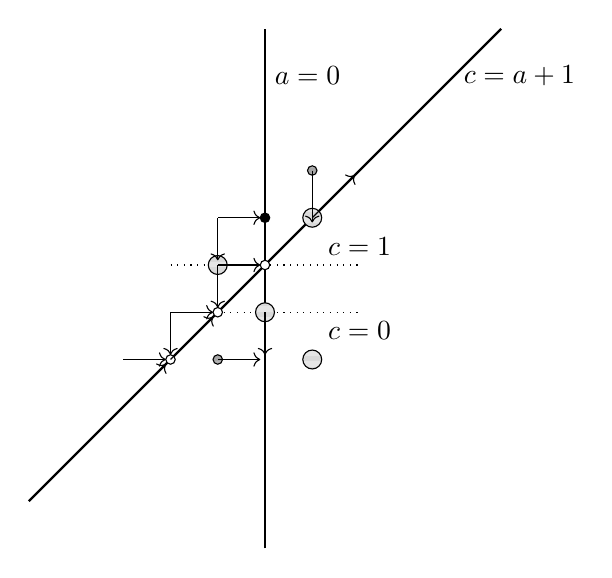
\begin{tikzpicture}[scale=0.6]
\draw (0,5) node[right]{$a=0$};
\draw[thick,black] (0,-5)--(0,6);

\draw (4,5) node[right]{$c=a+1$};
\draw[thick,black] (-5,-4)--(5,6);

\draw(2,0) node[below]{$c=0$};
\draw[dotted] (-2,0)--(2,0);

\draw(2,1) node[above]{$c=1$};
\draw[dotted] (-2,1)--(2,1);

\filldraw [pattern=horizontal lines gray] (-1,-1) circle (0.1);
\filldraw [pattern=horizontal lines gray] (1,-1) circle (0.1);
\filldraw [fill=white] (-2,-1) circle (0.1);

\filldraw [fill=white] (-1,0) circle (0.1);
\filldraw [fill=black] (0,0) circle (0.1);

\filldraw [pattern=horizontal lines gray] (-1,1) circle (0.1);
\filldraw [fill=white] (0,1) circle (0.1);

\filldraw [fill=black] (0,2) circle (0.1);
\filldraw [fill=white] (1,2) circle (0.1);

\filldraw [pattern=horizontal lines gray] (1,3) circle (0.1);

\filldraw [pattern=horizontal lines light gray] (1,-1) circle (0.2);
\filldraw [pattern=horizontal lines light gray] (0,0) circle (0.2);
\filldraw [pattern=horizontal lines light gray] (-1,1) circle (0.2);
\filldraw [pattern=horizontal lines light gray] (1,2) circle (0.2);

%% 同型矢印
\draw[->] (-3,-1)--(-2-0.1,-1);
\draw[->] (-1,-1)--(0-0.1,-1);

\draw[->] (-2,0)--(-2,-1+0.1);
\draw[->] (-2,0)--(-1-0.1,0);
\draw[->] (0,0)--(0,-1+0.1);
%\draw[->] (1,0)--(1,-1+0.1);

\draw[->] (-1,1)--(0-0.1,1);
\draw[->] (-1,1)--(-1,0+0.1);
%\draw[->] (1,1)--(1,0+0.1);
%\draw[->] (1,1)--(2,1);
%\draw[->] (2,1)--(2,2-0.1);

\draw[->] (-1,2)--(-1,1+0.1);
\draw[->] (-1,2)--(0-0.1,2);

\draw[->] (1,3)--(1,2-0.1);

%% 追加
\draw[->] (1,2)--(2-0.1,3-0.1);
\draw[->] (-2,-1)--(-1-0.1,0-0.1);
\draw[->] (-3,-2)--(-2-0.1,-1-0.1);
\end{tikzpicture}
\end{center}
\caption{A part of the directed graph and reducing representatives}
\label{fig:directed-graph-1F1}
\end{figure}

All set $I$ obtained by Algorithm \ref{alg:representative} for the system for ${}_1F_1$ are of mesh type and
Figure \ref{fig:directed-graph-1F1} illustrates a part of the directed graph
of isomorphisms.
Big circles of the figure are reduced set of representatives.
\end{example}


\begin{remark}\rm
%%Ref: 2025-07-24-resprentative-man.tex
Let $\{ L_i(s) \}$ be a set of linear polynomials of $d$-variables 
with integer coefficients.
We consider the arrangment defined by $\{ L_i(s)=0 \}$.
A problem of finding a Markov basis for the set 
$\{ s \in \ZZ^n \,|\, L_i(s) > 0 \mbox{ for all $i$}\}$
can be reduced to the method of finding a Markov basis
for the standard expression of the feasible points
$\{ u \in \NN_0^n \,|\, Au=b \}$
where $A$ is a matrix and $b$ is a vector with integer entries
(see, e.g., \cite{sturmfels-toric}).
We set $s=u-v \in \ZZ^d$, $u,v \in \NN_0^d$
and express the set as $\{ (u,v) \in \NN_0^{2d} \,|\, L_i(u-v) \geq 1 \}$.
Adding slack variables, we express the set in the $(u,v)$ space
as the standard expression of the feasible points.
Thus our reduction is done. 
A markov basis for the lattice points in a relative interior 
of a face of the arrangement can be obtained analogously.
%%todo, implementation.
\end{remark}

\begin{remark}\rm
The set $I$ can be regarded as feasible points of an integer program.
Then, the Markov basis that connects all points in $I$ can be obtained 
by a Gr\"obner basis with the trick in the previous remark.
%%Ref: 2025-07-24-resprentative-man.tex
If $I$ is not of mesh type,
we compute a Markov basis $\{ m_j \}$ and
contiguity relations for moves $\{ \pm m_j \}$.
We have new $b$-functions and the arrangement may become finer.  
We repeat this procedure until the arrangement does not become finer.
%%Ref: 2025-07-24-resprentative-man.tex
Although Saito proved isomorphic classes of $H_A(\beta)$
are finite when $\beta \in \ZZ^d$ \cite{saito-isom}, 
we cannot prove that this repetition stops in finite steps for now.
It is a future problem for us to study this method utilizing Markov bases.
\end{remark}



\begin{theorem}
If $A=(E,*)$ is normal, we can classify the associated Horn systems $H_A(\beta)$ 
for $\beta \in \ZZ^d$
into isomorphic classes and compute contiguity relations among isomorphic
systems.
\end{theorem}

\begin{proof}
We denote the GKZ hypergeometric by the same symbol $H_A(\beta)$.
Let $F_\sigma(s)$ be the primitive integral supporting function
where  $\sigma$ is a facet of the cone generated 
by the column vectors of $A$.
Since $\beta, \beta' \in \ZZ^d$,
the values of $F_\sigma(\beta)$ and $F_\sigma(\beta')$ belong to $\ZZ$.
Consider the hyperplane arrangement ${\cal A}$
defined by $F_\sigma(s)=0$ where $\sigma$ runs over the facets.
Assume that $\beta$ and $\beta'$ belong to the relative interior of a same face of the arrangement.
It follows from \cite[Th. 5.2]{saito-isom} that
$M_A(\beta):=D/H_A(\beta)$ and $M_A(\beta')$ are isomorphic,
because the theorem says that they are isomorphic 
if and only if $\beta-\beta' \in \ZZ A$
and
$$
 \{ \mbox{facet $\sigma$} \,|\, F_\sigma(\beta) \in \NN_0 \}
=
 \{ \mbox{facet $\sigma$} \,|\, F_\sigma(\beta') \in \NN_0 \}.
$$

Compute a Markov basis for the lattice points in the relative 
interior of each face of the arrangement ${\cal A}$
and contiguity relations associated to the basis.
Note that contiguity relations can always be found
because $M_A(\beta)$ and $M_A(\beta')$ are isomorphic
(Section \ref{sec:rat-sol}).
It follows from Theorem \ref{th:bf_for_A}, Section \ref{sec:restriction_of_A_hg}
and 
that the isomorphism among $M_A(\beta)$ and $M_A(\beta')$ 
gives an isomorphism among associated Horn systems
that we have completed the proof.
\end{proof}

\section{Comprehensive Restriction Algorithm} \label{sec:restriction}

Let $D_n$ be the Weyl algebra of $n$ variables.
Let $I(\kappa)$ be a holonomic left ideal of $D_n$ 
with parameters $\kappa \in \CC^d$.
We want to compute the restriction module
\begin{equation}  \label{eq:restriction_module}
 \frac{D_n}{I(\kappa)+x_1 D_n + \cdots + x_m D_n}.
\end{equation}

\begin{algorithm}{\rm (Comprehensive restriction algorithm that gives 
a partial answer)}   \label{alg:alg-rest-top} \rm
\begin{itemize}
\item Input: $I(\kappa)$, $x_1=\cdots=x_m=0$. 
\item Output: Strata $S_1$, $S_2$ and $S_3$ of the $\kappa$ space $\CC^d$.
The restriction module (\ref{eq:restriction_module}) on each stratum of them. 
\end{itemize}
\begin{enumerate}
\item {\tt Ans=[\,]}.
\item Put $w=(\overbrace{1,\ldots,1}^{m}, 0, \ldots, 0)$ and compute
a comprehensive Gr\"obner system $G$ by \, $\prec_{(-w,w)}$ order.
\item Compute comprehensive $b$-functions for restriction, which are monic generators
of \, ${\rm in}_{(-w,w)}(I(\kappa)) \cap \CC[\theta_1+\cdots+\theta_m]$.
Let $S_1$ be strata of the comprehensive $b$-functions that refines strata 
of the comprehensive Gr\"obner system.
\item For each stratum $U$ of $S_1$, refine $U$ into subsets such that 
(a) the maximal non-negative integral root
of the $b$-function is $0$ or (b) no non-negative integral root of $b$ or (c) other cases on each subset.
Let $S_2'$ be the collection of subsets such that (a) or (b) holds.
Let $S_3'$ be the collection of subsets such that (c) holds.
\item For each stratum $V$ of $S_2'$,
compute a comprehensive Gr\"obner system of $G''=G'|_{x_1=\cdots=x_m=0}$
where $G'$ is the collection of the elements of the $(-w,w)$ Gr\"obner basis $G$
on $V$
such that ${\rm ord}_{(-w,w)}(g) \leq 0$,  $g \in G$.
It refines $V$ and let $S_2$ be the collection of these refinement.
\begin{enumerate}
\item The restriction module on each stratum $W$ of $S_2$ of type (a) is
$\frac{D'}{\left\langle \mbox{\rm (a Gr\"obner basis of $G''$ on $W$)} \right\rangle}$
where $D'=\CC\langle x_{m+1}, \ldots, x_n, \pd{m+1}, \ldots, \pd{n} \rangle$.
Append them to {\tt Ans}.
\item The restriction module (output) is $0$ on the set of strata of $S_2'$ of type (b). Append them to {\tt Ans}.
\end{enumerate}
\item For $V$ in $S_3'$ (type (c)), 
if $I(\kappa)$, $\kappa \in V$ is a GKZ system or a hypergeometric system of Horn type discussed in previous sections, 
call 
\, {\tt Rfr}($I(\kappa(p)), p,G, V)$ (\underline{r}epresentatives \underline{f}or \underline{r}estriction, Algorithm \ref{alg:hg-rest})
where we reparametrize $\kappa$ by $p$ as $\kappa_i(p)=p_i$.
The return value is strata $S_3$ and restrictions on each stratum of $S_3$.
Append them to {\tt Ans}.
If $I(\kappa)$ does not belong to these hypergeometric systems, this algorithm
does not give an answer.
\item Return {\tt Ans}.
\end{enumerate}
\end{algorithm}

\begin{example}\rm
Let $\kappa=(a,b,c) \in \CC^3$
and consider the left ideal $I(\kappa)$ of $D_1$
generated by the Gauss hypergeometric operator
$ L=x(1-x)\p^2 + (c - (a + b + 1)x)\p - ab $.
Here $x_1$ is denoted by $x$ and $\pd{1}$ by $\p$.
The set $\{L\}$ is $(-1,1)$ Gr\"obner basis for any $\kappa$.
Then $S_1 = \{ \CC^3 \}$.
We have ${\rm in}_{(-1,1)} (L)= x \p^2 + c \p$,
then the $b$-function for restriction is $\theta_1 (\theta_1+c-1)$.
Then $S_2'$ is $\{ V \}$ where
$V=\{ (a,b,c) \,|\, c \not\in \ZZ_{\leq 0} \}$.
Since ${\rm ord}_{(-1,1)}(L)=1$, we have $G'=\emptyset$.
Then the restriction module on $V$ is $D'=\CC$.
The strata $S_3'$ (case (c)) is $\{W\}$ where 
$W=\{ (a,b,c) \,|\, c \in \ZZ_{\leq 0} \}$.
This case will be discussed in Section \ref{sec:gauss-hg}.
\end{example}

Let ${\bar q}_1$ be the maximal non-negative integral root
of the $b$-function for the restriction.
Let $G$ be the $G$ that appears in Algorithm \ref{alg:alg-rest-top}.
We denote by 
$\mbox{\tt Rest}(G,{\bar q}_1)$
the output of the final step of 
computing Gr\"obner basis in a free module
of the restriction algorithm, see, e.g.,
\cite[Steps 6 and 7 of Alg. 5.2.8]{SST}.
Since $G$ contains parameters, the return value is 
a comprehensive Gr\"obner system consisting of a strata and
Gr\"obner basis on each stratum.

\begin{example} \rm
Let $H_2(a,b,b',c,c')$ be the left ideal
generated by (\ref{eq:f2a}) and (\ref{eq:f2b})
that annihilates the Appell function $F_2$.
Consider the left $D_2$-module $M(a,b,b',c,c')=D_2/H_2(a,b,b',c,c')$.
Suppose that $c=0$ and $c' \notin \ZZ_{\leq 0}$.
The maximum non-negative root of the $b$-function is $s_0=1-c=1$
(see Example \ref{ex:f1-f2-comprehensive-b-fn}).
%%Ref: appell2_ja.tex
The restriction module is
$$
\frac{\CC\pd{x}+\CC\pd{y}+\CC}
 {
   \CC (-a b) + \CC c' \pd{y} + \CC (-a b')
 }.
$$
The dimension is equal to $3$ minus the rank of the matrix
$$
\begin{pmatrix}
0 & 0 & -\aalpha \bbeta \\
0 & \ggamma' & -\aalpha \bbeta' 
\end{pmatrix}.
$$
The stratification with respect to the rank can be obtained
by a comprehensive Gr\"obner system for linear polynomials.
$\mbox{\tt Rest}(G,1)$ returns this comprehensive Gr\"obner basis.
\end{example}


In order to compute the restriction modules on the strata $S_3'$
for a GKZ system or for a hypergeometric system of Horn type, 
we apply the following algorithm utilizing algorithms to find contiguity relations.
This algorithm is a variation of {\tt representative\_candicate} \ 
(Algorithm \ref{alg:representative}).

\begin{algorithm} \label{alg:hg-rest} \rm
Procedure $\mbox{\tt Rfr}(H_A(\beta(p),p,G',E)$. \quad \\
Input: $H_A(\beta(p))$ (hypergeometric system), $p$ (a set of $m$ parameters), 
$G'$ ($(-w,w)$-Gr\"obner basis), $E$ (conditions). \\
%% E is equality constraints.
Output: a list of [conditions(stratum), restriction, contiguity relations].
\begin{enumerate}
\item {\tt Ans=[\,]}.
\item Let $r_1(p), \ldots, r_k(p)$ be the roots
of the $b$-function for the restriction.
\item For all $r_i$, assume $r_i \in \ZZ_{\geq 0}$ or not
and relationships (larger or smaller or equal)
among $r_i$'s supposed to be non-negative integers.
Let $\tilde K$ be the set of all distinct assumptions
on $r_i$'s.
\item For $K \in {\tilde K}$ do
\begin{enumerate}
\item $q(p)$ be the maximal non-negative integral root under the assumption $K$.
If $q(p)$ is a constant, append
$[E \cap K, \mbox{\tt Rest}(G,q(p)), \emptyset]$ to {\tt Ans}
and continue the for-loop.
\item Changing the indexing, 
we suppose that $q(p)$ depends on $p_1$.
Introduce new variables $q_1, \ldots, q_m$
such that
$q_1 = q = \alpha p_1 + \cdots$ ($\alpha \not= 0$),
$q_i=p_i$ ($i \geq 2$)
and express $\beta$ by $q$.
\item Choose $\delta \in \ZZ_{>0}$ so that
\begin{equation}
 \beta_i(q+\delta e_1)-\beta_i(q) \in \ZZ \quad
\mbox{for all $i$}
\end{equation}
where $e_1=(1,0, \ldots, 0)$.
\item Put $\Lambda = \{0, 1, 2, \ldots, \delta-1\}$.
\item For $k$ in $\Lambda$ do
\begin{enumerate}
\item Derive the contiguity relation for it $(L_u, L_d, b(q))$
\begin{equation}
  D/H_A(\beta(q+k e_1))
\stackrel{L_d}{\rightarrow}
  D/H_A(\beta(q+(k+\delta)e_1))
\stackrel{L_u}{\rightarrow}
  D/H_A(\beta(q+k e_1))
\end{equation}
where $ L_d L_u \equiv b(q)$.
\item Consider 
\begin{equation}  \label{eq:segments}
 \left( \RR^m \setminus V(b) \right) \cap
 \left( \RR \times ({\bar q}_2, \ldots, {\bar q}_m) \right)
\end{equation}
where ${\bar q}_2, \ldots, {\bar q}_m$ are generic numbers.
Let $Q$ be the set of the $q_1 \in \NN_0$ that is the minimum 
in each first coordinate of connected components
of (\ref{eq:segments}).
\item Factorize $b(q)$ into degree $1$ polynomials as $\prod_{j=1}^J b_j(q)$.
\item For all ${\bar q}_1 \in Q$ do
\begin{enumerate}
\item Append $[E \cap K \cap \{ b(q)\not=0 \}, \mbox{\tt Rest}(G,{\bar q}_1),\mbox{the contiguity relation}]$.
\end{enumerate} 
\item For all factors $b_j$ in $b$ do
\begin{enumerate}
\item Eliminate one variable in $q_1, \ldots, q_m$ by $b_i(q)=0$.
Changing indices, we suppose that $q_m$ is eliminated.
\item Express $\beta$ in terms of $q_1, \ldots, q_{m-1}$.
\item Append \, $\mbox{\tt Rfr}(H_A(\beta(q_1, \ldots, q_{m-1}),
(q_1, \ldots, q_{m-1}), G, E \cap K \cap \{b_i=0\})$
to {\tt Ans}.
\end{enumerate}
\end{enumerate}
\end{enumerate}
\item Return {\tt Ans}.
\end{enumerate}
\end{algorithm}

\begin{remark}\rm
Although, as long as we have tried, we can always find a contiguity
relation of $\delta e_1$ shift,
we might fail at this step.
If we fail to find a contiguity relation of $\delta e_1$ shift,
we need to increase $\delta$.
Since the number of isomorphic classes of $H_A(\beta+\iota)$, $\iota \in \ZZ^d$
are finite by \cite{saito-isom}, we can find a contiguity relation
at a suitable $\delta e_1$.
\end{remark}

\begin{remark}\rm
Algorithms \ref{alg:alg-rest-top} and \ref{alg:hg-rest} 
will be generalized to obtain
a restriction complex (a restriction of $D_n/I(\kappa)$ in a derived category)
by applying the algorithm of \cite{OT-rest}.
Note that we need to replace ``maximal non-negative integral root''
of the algorithms \ref{alg:alg-rest-top} and \ref{alg:hg-rest}
by ``maximal integral root''.
A comprehensive version of $(-w,w)$-adapted resolution is an open question
to give an algorithm to obtain a restriction complex.
\end{remark}

\begin{example}\rm \label{ex:1F1-restriction}
This is a continuation of Example \ref{ex:1F1} (${}_1 F_1$ case).
The $b$-function for the restction to $x=0$
is $s(s+c-1)$.
The roots are $s=0$ and $s=1-c$.
Type (a) case is $1-c \not\in \ZZ_{\geq 0}$.
Since ${\rm ord}_{(-1,1)}(L)=1$, $G''$ is empty.
Then the restriction is $\CC$.
Since $s$ is a factor of the $b$-function, type (b) case does not occur.


Consider the type (c) case.
In other words, assume $c \in \ZZ_{\leq 1}$.
Let this assumption be $E$.
$G$ is $\{ L \}$.
We call the procedure 
$\mbox{\tt Rfr}(H_A((a,c)), (a,c), G, E)$.
Put $q_1=1-c$ and $q_2=a$.
Then, $\Lambda=\{ 0 \}$.
The condition on $c$ becomes $q_1=1-c \in \ZZ_{\geq 1}$
and the roots of the $b$-function for restriction is $0$ and $q_1$.
Firstly, we compute 
a contiguity relation for the shift from $q_1=1-c$ to $q_1+1=1-(c-1)$.
The $b$-function for contiguity is $q_1+q_2=1-c+a$
by (\ref{eq:conti-bf-1F1-c}).
$\left( \RR^2 \setminus V(q_1+q_2) \right) \cap \left( \RR \times {\bar q}_2 \right)$ 
is $ (-\infty,\infty) \times {\bar q}_2$.
Then the set $Q$ of the minimal non-negative integers in the connected component is $\{ 0 \}$.
The restriction on this stratum is isomorphic to that of $D/H_A((a,c)=(a,0))$.
Since the maximal integral root is $1$ in the $(a,c)$ parameter space
and ${\rm ord}_{(-1,1)}(L)=1$,
we have $G''=\{ L|_{x=0}= -a \}$.
Thus, the restriction is $\CC$ when $a \not= 0$
and is $\CC^2$ when $a=0$.
%%Prog: rest-comprehensive4/Data/2025-08-07-rest-1F1.rr
Secondly, we consider the case $q_1+q_2 = 1-c+a=0$.
The parameter space is one dimensional and parametrized as
$(a,c)=(0,1)-(1,1)s'$.
We call the procedure
$\mbox{\tt Rfr}(H_A((-s',1-s')), s', G, \{ c \in \ZZ_{\leq 0}, c=a+1=-s'+1 \}$.
The $b$-function for the contiguity
of the shift $s' \mapsto s'+1 \mapsto s'$ 
is $s'(s'-1)=c(c-1)$.
Then, the cases of $s'=\{ -1,0,1 \}$ are representatives
of isomorphic classes.
In other words, $(a,c)=(1,2), (0,1), (-1,0)$ are the representatives. 
%%Prog: 2025-08-07-rest-1F1.rr,  2025-08-07-1F1-special-sol.pdf (by Mathematica).
The restrictions are all $\CC$. 
\end{example}


This procedure will be a little complicated.
Then, more examples will help.
The comprehensive restriction algorithm will be illustrated for
the Gauss hypergeometric system and the system of Appell function 
$F_1$ 
in the following sections \ref{sec:gauss-hg} and \ref{sec:f1}. 


\section{Restriction of the Gauss Hypergeometric System to the Origin} \label{sec:gauss-hg}
%%macros \aalpha, \bbeta, \ggamma are used.

The Gauss hypergeometric function ${}_2F_1(a,b,c;x)$ is annihilated by
the operator
\begin{equation} \label{eq:gauss_hg_op}
L(\aalpha, \bbeta, \ggamma) = x(1-x)\pd{x}^2 + (\ggamma - (\aalpha + \bbeta + 1)x)\pd{x} - \aalpha \bbeta.
\end{equation}
We consider the left ideal generated by $L$
$$
\Hg(\aalpha, \bbeta, \ggamma) = D L(\aalpha, \bbeta, \ggamma)
$$
where $D=D_1$.
We will compute the restriction module
$$M(\aalpha, \bbeta, \ggamma)/xM(\aalpha, \bbeta, \ggamma) \cong D/(\Hg(\aalpha, \bbeta, \ggamma) + x D)$$ 
of the left $D$-module $M(\aalpha, \bbeta, \ggamma) = D/\Hg(\aalpha, \bbeta, \ggamma)$
to $x = 0$.

The generic $b$-function (for restriction)
is 
$$
b(s) = s(s+\ggamma-1)
$$
with respect to the weight vector $w=(1)$.
The stratum for this $b$-function is 
$\CC^3=\{ (\aalpha, \bbeta, \ggamma) \in \CC^3 \}$.
The maximal non-negative integral root $s_0$ of
$b(s)$ is
$$
s_0 = 
\begin{cases}
0 & (\ggamma \notin \mathbb{Z}_{\leq 0}) \\
1-\ggamma & (\ggamma \in \mathbb{Z}_{\leq 0}).
\end{cases}
$$

The Gr\"obner basis $G$ of $\Hg$ by Algorithm \ref{alg:alg-rest-top}
is $\{ L \}$.
The case (b) does not occur and the stratification $S_2$
of the case (a) consists of only one stratum
$$
 \{ (\aalpha,\bbeta,\ggamma) \,|\, \ggamma \notin \mathbb{Z}_{\leq 0} \}
$$
and the restriction module is isomorphic to $\mathbb{C}$,
because ${\rm ord}_{(-w,w)}(L)=1$ and then $G''=\emptyset$.

Before illustrating steps of the procedure 
$\mbox{\tt Rfr}(\Hg,(\aalpha,\bbeta,\ggamma),G,\ggamma \in \mathbb{Z}_{\leq 0})$,
we show a conclusion that is a list of the restrictions depending on $\ggamma$. 
\begin{enumerate}
\item[(1)]
When $\ggamma \notin \mathbb{Z}_{\leq 0}$,
the restriction module is isomorphic to $\mathbb{C}$.

\item[(2)]
Suppose that $\ggamma = 0$. 
%%%%%%%%%%%%%%%%%%%%%%%%%%%%%%%%%%%%%%%%%%%%%%%%%%%%%%%%%%%%%
\if 0
%%Prog: restriction([gauss(a,b,0)], next lines.
[4436] nk_restriction.restriction([gauss(a,b,0)], [x], [dx], [1]|param=[a,b]);
-- nd_weyl_gr :0sec(0sec)
-- weyl_minipoly_by_elim :0sec(0sec)
-- generic_bfct_and_gr :0sec(0sec)
generic bfct : [[-1,1],[s,1],[s-1,1]]
S0 : 1
B_{S0} length : 2
-- fctr(BF) + base :0sec(0sec)
[[-b*a],[[1],[0]]]
\fi
%%%%%%%%%%%%%%%%%%%%%%%%%%%%%%%%%%%%%%%%%%%%%%%%%%%%%%%%%%%%%
We have $s_0 = 1$ and then $\mathcal{B}_1 = \{1, \p_x\}$ 
(see, e.g., \cite[Alg. 5.2.8]{SST}).
Consider the $\mathbb{C}$-vector space with a basis $\mathcal{B}_1$
$\mathbb{C}^2 = \mathbb{C} \cdot 1 + \mathbb{C} \cdot \p_x$.
Sorting the terms in $L(\aalpha, \bbeta, 0)$ by $<_{(-1,1)}$,
we have
$$
L(\aalpha, \bbeta, 0) = 
x \p_x^2 - x^2 \p_x^2 + (-\aalpha - \bbeta - 1 ) x \p_x - \aalpha \bbeta.
$$
Since the $(-1,1)$-degree of it is $1$, the vector space 
of the denominator of the restriction module is generated by
$(L(\aalpha, \bbeta, 0))|_{x=0}$ 
that is
$$
(L(\aalpha, \bbeta, 0))|_{x=0} = -\aalpha \bbeta .
$$
Thus, the restriction module is 
$\mathbb{C}^2/V$ where 
$
V = \mathbb{C} \cdot \aalpha \bbeta 
$.
Therefore, we have two cases as
  \begin{itemize}
   \item
   When $\aalpha = 0$ or $\bbeta = 0$, $V=\{0\}$ and the restriction module is 
a $2$-dimensinal vector space $\mathbb{C}^2$.
   \item
   When $\aalpha \neq 0$ and $\bbeta \neq 0$, $V=\mathbb{C}$  and the restriction module is a $1$-dimensional vector space $\mathbb{C}$.
   \end{itemize}
%
\item[(3)]
When $\ggamma \in \mathbb{Z}_{< 0}$,
we can reduce cases of 
$\ggamma \in \mathbb{Z}_{< 0}$ to the case of $\ggamma = 0$
by utilizing left $D$-module isomorphism
$$
D/\Hg(\aalpha, \bbeta, \ggamma) \cong D/\Hg(\overline{\aalpha}, \overline{\bbeta}, \ggamma+1)
$$ 
where 
$\overline{\aalpha}, \overline{\bbeta}$ are 
$\aalpha$ or $\aalpha+1$ and $\bbeta$ or $\bbeta+1$ respectively.
We will prove this fact in Proposition \ref{prop:c-isom-gauss-hg}
\end{enumerate}

Note that we do not give a stratification of 
$\{(\aalpha,\bbeta,\ggamma)\,|, \ggamma \in \mathbb{Z}_{<0}\}$
in the last claim above.
We will discuss on it after the proposition.

\begin{proposition} \label{prop:c-isom-gauss-hg}
When $\ggamma \in \mathbb{Z}_{< 0}$,
$$D/\Hg(\aalpha, \bbeta, \ggamma) \cong D/\Hg(\overline{\aalpha}, \overline{\bbeta}, 0)$$ 
holds
where 
$\overline{\aalpha}, \overline{\bbeta}$ are 
$\aalpha$ or $\aalpha+1$ and $\bbeta$ or $\bbeta+1$ respectively.
\end{proposition}

\begin{proof}
We abbreviate the Gauss hypergeometric operator as
$L(\ggamma) = L(\aalpha, \bbeta, \ggamma)$
and the left ideal generated by $L$ as 
$\Hg(\ggamma) = \Hg(\aalpha, \bbeta, \ggamma)$. 

The down-step operator $B(\ggamma)$ with respect to $\ggamma$
satisfies
$$\exists P \in D ~{\rm s.t.}~ L(\ggamma-1) B(\ggamma) = P L(\ggamma). $$
The operator
$$
B(\ggamma) = \theta_x +  (\ggamma - 1)
$$
satisfies it.
The up-step operator $H(\ggamma)$ satisfies 
$$L(\ggamma+1) H(\ggamma) = P L(\ggamma).$$
The operator
$$
\Hg(\ggamma) =  (1-x) \p_x + (\ggamma-\aalpha-\bbeta)
$$
satisfies it.

Composing left $D$-module homomorphisms
$$
\varphi : D/\Hg(\ggamma+1) \ni [P] \mapsto [P \cdot H(\ggamma)] \in D/\Hg(\ggamma)
$$
$$
\psi : D/\Hg(\ggamma) \ni [P] \mapsto [P \cdot B(\ggamma+1)] \in D/\Hg(\ggamma+1),
$$
we have
$$
\varphi \circ \psi : D/\Hg(\ggamma) \ni [P] \mapsto [P \cdot B(\ggamma+1) \cdot H(\ggamma)] \in D/\Hg(\ggamma)
$$ 
$$
B(\ggamma+1) \cdot H(\ggamma) \equiv (\aalpha-\ggamma)(\bbeta-\ggamma) ~{\rm mod}~  \Hg(\ggamma)
$$
$$
\varphi \circ \psi = (\aalpha-\ggamma)(\bbeta-\ggamma) {\rm id}.
$$
Reversing the order of the composition,
we have
$$
\psi \circ \varphi : D/\Hg(\ggamma+1) \ni [P] \mapsto [P \cdot H(\ggamma) \cdot B(\ggamma+1)] \in D/\Hg(\ggamma+1)
$$
$$
H(\ggamma) \cdot B(\ggamma + 1) \equiv (\aalpha-\ggamma)(\bbeta-\ggamma) ~{\rm mod}~  \Hg(\ggamma+1)
$$
$$
\psi \circ \varphi  = (\aalpha-\ggamma)(\bbeta-\ggamma)  {\rm id}. 
$$
Hence, when 
$(\aalpha - \ggamma)(\bbeta - \ggamma) \neq 0$,
we have the isomorphism 
$
D/\Hg(\aalpha, \bbeta, \ggamma) \cong D/\Hg(\aalpha, \bbeta, \ggamma+1)
$.

The isomorphism breaks when
$$\aalpha - \ggamma = 0 \text{ or } \bbeta - \ggamma = 0.$$
We derive contiguity relations with respect to $\ggamma$ 
for these cases.

\begin{itemize}
\item[(1)] When $\aalpha - \ggamma = 0$,
put $\aalpha = \ggamma$.
The up-step and down-step operators
for $\Hg(\ggamma, \bbeta, \ggamma)$ with respect to $\ggamma$ 
are
\begin{align*}
&B(\ggamma) = (1-\ggamma)(x(x-1) \p_x +\bbeta x - \ggamma + 1), \\
&H(\ggamma) = (x-1) \p_x + \ggamma, \\
&B(\ggamma+1) \cdot H(\ggamma) \equiv \ggamma^2 (\bbeta - \ggamma) ~{\rm mod}~ \Hg(\ggamma+1), \\
&H(\ggamma) \cdot B(\ggamma+1) \equiv \ggamma^2 (\bbeta - \ggamma) ~{\rm mod}~ \Hg(\ggamma).
\end{align*}
Hence, when $\ggamma^2 (\bbeta - \ggamma) \neq 0$,
$D/\Hg(\ggamma, \bbeta, \ggamma) \cong D/\Hg(\ggamma+1, \bbeta, \ggamma+1)$
holds. 

\item[(1-1)] When $\bbeta - \ggamma = 0$,
put $\bbeta = \ggamma$.
The up-step and down-step operators for  $\Hg(\ggamma, \ggamma, \ggamma)$
with respect to $\ggamma$ are
\begin{align*}
&B(\ggamma) = (1-\ggamma)(x(x-1) \p_x + (2\ggamma-1)x - \ggamma+1), \\
&H(\ggamma) = \p_x, \\
&B(\ggamma+1) \cdot H(\ggamma) \equiv \ggamma^3 ~{\rm mod}~ \Hg(\ggamma+1), \\
&H(\ggamma) \cdot B(\ggamma+1) \equiv \ggamma^3  ~{\rm mod}~ \Hg(\ggamma).
\end{align*}
Hence, when $\ggamma^3 \neq 0$,
$D/\Hg(\ggamma, \ggamma, \ggamma) \cong D/\Hg(\ggamma+1, \ggamma+1, \ggamma+1)$
holds.

\item[(2)] When $\bbeta - \ggamma = 0$,
put $\bbeta = \ggamma$.
The up-step and down-step operators for $\Hg(\aalpha, \ggamma, \ggamma)$
with respect to $\ggamma$ are
\begin{align*}
&B(\ggamma) = (1-\ggamma)(x(x-1) \p_x +\aalpha x - \ggamma + 1), \\
&H(\ggamma) = (x-1) \p_x + \ggamma, \\ 
&B(\ggamma+1) \cdot H(\ggamma) \equiv -\ggamma^2 (\aalpha - \ggamma) ~{\rm mod}~ \Hg(\ggamma+1), \\
&H(\ggamma) \cdot B(\ggamma+1) \equiv -\ggamma^2 (\aalpha - \ggamma) ~{\rm mod}~ \Hg(\ggamma).
\end{align*}
When $\ggamma^2 (\aalpha - \ggamma) \neq 0$,
$D/\Hg(\aalpha, \ggamma, \ggamma) \cong D/\Hg(\aalpha, \ggamma+1, \ggamma+1)$
holds. 

\item[(2-1)] The case $\aalpha - \ggamma = 0$ 
is reduced to the case 1-1.
\end{itemize}
\end{proof}

\begin{example}\rm \label{ex:2F1-Rfr}
%% We use a,b,c instead of (\aalpha,\bbeta,\ggamma)
Let us illustrate the behavior of $\mbox{\tt Rfr}(\Hg(\beta),p=(a,b,c),G,I)$
where $\beta=(a,b,c)$,
$G=\{ L \}$ and the condition $I$ is $c \in \ZZ_{\leq 1}$.
We retain symbol names of Algorithm \ref{alg:hg-rest}
and of the proof of Proposition \ref{prop:c-isom-gauss-hg}.
The roots of the $b$-function for restriction
are $r_1=0$ and $r_2=1-c$.
Under the assumption $I$, we have $r_2 \geq r_1$.
Then we put
$$ 
 q_1(p)=1-c, q_2(p)=a, q_3(p)=b. 
$$
We can set $\delta=1$ and then $\Lambda=\{ 0 \}$.
The contiguity relation is 
$(B(c), L(c+1), (a-c)(b-c))$.
The $b$-function of contiguity
$(a-c)(b-c)$ can be written in terms of $q$ as
$b(q)=(q_1+q_2-1)(q_1+q_3-1)$.
If $q_2$ and $q_3$ are generic numbers,
there is only one connected component
of (\ref{eq:segments}).
The first coordinate of it is $(-\infty,\infty)$.
Then, the minimum is $0$ which means
$c=1$ ($q_1=0$).
Hence, the restriction module is $\CC$ 
when $c \in \ZZ_{\leq 1}$ and $(a-c)(b-c)\not=0$.
Isomorphisms are given by the contiguity relation.

Let us run $\mbox{\tt Rfr}$ recursively with fewer parameter degrees of freedom.
Let $b_1(q)$ be $q_1+q_3-1$.
We eliminate $q_3$ by $b_1(q)=0$ ($b=c$) and we call
$$
 \mbox{\tt Rfr}(\Hg(q_2,1-q_1,1-q_1),(q_1,q_2),G,
  q_1 \in \ZZ_{\geq 0} \ \mbox{ and }\ q_1+q_3-1=0).
$$
Note that $(q_2,1-q_1,1-q_1)=(a,c,c)$.
Let us execute this procedure.
The roots of $b$-function for restriction is $0$ and $q_1$.
The $\delta$ is $1$ and $\Lambda=\{ 0 \}$.
As we have seen in the proof of Proposition \ref{prop:c-isom-gauss-hg},
the contiguity relation is
$$
\left(
 (x-1)\pd{}+c,
 (1-c)\left( x(x-1)\pd{} + ax - c +1 \right),
 -c^2(a-c)
\right) 
$$
where $-c^2(a-c)=-(1-q_1)^2(q_1+q_2-1)$.
Assume that $q_2=a:={\bar q}_2$ is a generic number.
The connected component of (\ref{eq:segments})
are
$$
(-\infty,1) \times {\bar q}_2, \quad (1,\infty) \times {\bar q}_2.
$$
Then, $Q=\{ 0, 2 \}$.
When $q_1=0$ ($c=1$), the restriction module for $\Hg(a,1,1)$
is a representative of the isomorphic class consisting of $q_1=\{0\}$
and is $\CC$.
When $q_1=2$ ($c=-1$), the restriction module for $\Hg(a,-1,-1)$
is a representative of the isomorphic class consisting of $q_1=\{2,3,\ldots\}$.
Since $s_0=2$ in this case,
the restriction module is
$$
\frac{\CC + \CC \pd{} + \CC \pd{}^2}
 { \langle L|_{x=0}, :\pd{}L: |_{x=0} \rangle }
= \frac{\CC + \CC \pd{} + \CC \pd{}^2}{\CC \pd{}} 
\simeq \CC^2
$$
where $: \ : $ denotes the normally ordered expression
(see, e.g., \cite[p.3]{SST}).
%%Prog: 2025-08-12-rest-2F1.rr  R3
Since the $b$-function for the restriction is 
$-c^2(a-c)=-(1-q_1)^2 (q_1+q_2-1)$,
we need to call recursively $\mbox{\tt Rfr}$
for each factor.
For example, for the factor $1-q_1$,
we call the procedure for
$\Hg(a,0,0)$.
The $b$-function for this contiguity is $a(a+1)$.
Note that the degree of freedom of the parameters decreases when the recursion depth increases.
%%Prog: 2025-04-01-contiguity.rr gauss_contiguity_by_GKZ([a,0,0],[a+1,0,0]) and gauss_contiguity_by_GKZ([a+1,0,0],[a,0,0])

We believe that these explain how this process works, so we will skip the rest.
\end{example}

%\input gauss_hg_ja
\section{Restriction of Appell $F_1$ System to the Origin} \label{sec:f1}

Applying methods discussed in previous sections,
we obtain the following theorem.

\begin{theorem}
The restrictions of the hypergeometric system for the Appell function $F_1$
to $x=y=0$ are as follows.
They are $\CC$-vector spaces.
\begin{itemize}
\item 
When $\ggamma \notin \mathbb{Z}_{\leq 0}$, it is $\mathbb{C}$.

\item 
When $\bbeta = 0$ and $\bbeta' = 0$,
it is
$(\mathbb{C} \cdot 1 + \mathbb{C} \cdot \p_x + \mathbb{C} \cdot \p_y)$.

\item 
When ($\bbeta \neq 0$ or $\bbeta' \neq 0$) and $\aalpha = 0$,
it is
$(\mathbb{C} \cdot 1 + \mathbb{C} \cdot \p_x + \mathbb{C} \cdot \p_y)
/(\mathbb{C} \cdot (-\bbeta' \p_x + \bbeta \p_y)$ .

\item 
When ($\bbeta \neq 0$ or $\bbeta' \neq 0$) and $\aalpha \neq 0$,
it is
$(\mathbb{C} \cdot \p_x + \mathbb{C} \cdot \p_y)/
(\mathbb{C} \cdot (-\bbeta' \p_x + \bbeta \p_y))$.
\end{itemize}
\end{theorem}

Our proof is analogous to the case of the Gauss hypergeometric system.
Several contiguity relations are used.
They are obtained by our implementation
of our algorithms.
Our implementation and details of the proof are published 
in the internet\footnote{ 
\url{https://www.math.kobe-u.ac.jp/HOME/taka/2025/prog-rest}}.
The proof is omitted here.
% 英訳してこの論文に含めるのは2025/09の学会あとで. とりあえず日本語版を web に.
%


\if 0
% まだ英訳してない.
\input appell1_ja
\input appell2_ja
%\input appell2
\fi

\begin{thebibliography}{99}
%
\bibitem{barkatou-2012}
M.A.Barkatou, T.Cluzeau, C.El Bacha, J.-A.Weil,
Computing Closed Form Solutions of Integrable Connections,
ISSAC '12: Proceedings of the 37th International Symposium on Symbolic and Algebraic Computation, 43--50. \\
%% https://doi.org/10.1145/2442829.2442840
\url{https://www.unilim.fr/pages_perso/thomas.cluzeau/Packages/IntegrableConnections/PDS.html}
%
\bibitem{berkesch} C.Berkesch, L.F.Matusevich, U.Walther, 
Torus equivariant D-modules and hypergeometric systems, 
Advances in Mathematics, 350 (2019), 1226--1266.
%
\bibitem{bjork-2012}
J.E.Bj\"ork, Rings of differential operators, (2012), North Holland.
% ISBN 10 0444557180
%
\bibitem{not-2016}
K.Nabeshima, K.Ohara, S.Tajima, 
Comprehensive Gr\"{o}bner Systems in Rings of Differential Operators, 
Holonomic $D$-modules and $b$-functions,
ISSAC 2016 - Proceedings of the 2016 ACM International Symposium on Symbolic and Algebraic Computation,
349--356.
%%Ref: \url{https://doi.org/10.1145/2930889.2930918}
%
\bibitem{micciancio-2008}
D.Micciancio, Efficient reductions among lattice problems, 
%%DOI:10.1145/1347082.1347092, 
Proceedings of the Nineteenth Annual ACM-SIAM Symposium on Discrete Algorithms, SODA 2008, San Francisco, California, USA, January 20-22, 2008
%
\bibitem{nakayama-2024}
H.Nakayama,  Computing contiguity operators by Gr\"{o}bner bases of free modules,  
Suusikisyori 30(2) (2024), 3--8, (in Japanese).
\url{https://www.jssac.org/Editor/Suushiki/V30/No2/V30N2_102.pdf}
%
\bibitem{oaku-1997}
T.Oaku,
Algorithms for $b$-functions,
restrictions, and algebraic local cohomology groups of $D$-modules.
Advances in Applied Mathematics 19 (1997), 61--105.
%
\bibitem{OT-rest}
T.Oaku, N.Takayama,
Algorithms for $D$-modules -- restriction, tensor product, localization,
and algebraic local cohomology groups,
Journal of Pure and Applied Algebra
156 (2001), 267--308.
%
\bibitem{oshima-2012}
T.Oshima, Fractional calculus of Weyl algebra and Fuchsian differential equations, MSJ Memoirs, Mathematical Society of Japan, 28 (2012).
%
\bibitem{saito-isom}
M.Saito, Isomorphism Classes of $A$-Hypergeometric Systems,
Compositio Mathematica 128, (2001) 323--338.
%
\bibitem{SST}
M.Saito, B.Sturmfels, N.Takayama,
Gr\"obner Deformations of Hypergeometric Differential Equations, (2000), Springer.
%
\bibitem{SST-ip}
M.Saito, B.Sturmfels, N.Takayama,
Hypergeometric polynomials and integer programming.
Compositio Mathematica 155 (1999), 185--204. 
%
\bibitem{sturmfels-toric}
B.Sturmfels, Gr\"obner bases and convex polytopes,
AMS, 1996.
%
\bibitem{takayama-1989}
N.Takayama,
Gr\"obner basis and the problem of contiguous relations,  
Japan Journal of  Applied Mathematics, 
6 (1989), 147-160.
%
\bibitem{tw-hom}
H.Tsai, U.Walther, 
Computing homomorphisms between holonomic D-modules,
Journal of symbolic computation 32 (2001),  597--617.
%\url{https://doi.org/10.1006/jsco.2001.0485}.

%
\bibitem{weispfenning-1992}
V.Weispfenning, 
Comprehensive Gr\"obner bases, 
Journal of Symbolic Computation, 14 (1992), 1--29. 
%\url{https://doi.org/10.1016/0747-7171(92)90023-W}
\end{thebibliography}


\end{document}
